\documentclass[12pt,a4paper]{article}

% created by zcs at 2013-11-11
% Use XeLaTeX to compile.

% Package
\usepackage{amssymb}
\usepackage{fontspec}
\usepackage{xkeyval}
\usepackage[SlantFont,BoldFont,CJKchecksingle,CJKnumber]{xeCJK}
\usepackage{graphicx}
\usepackage{geometry}
\usepackage{fancyhdr}
\usepackage{lastpage}
\usepackage{indentfirst}
\usepackage{setspace}
\usepackage{titlesec}
\usepackage[normalem]{ulem}
\usepackage[CJKbookmarks]{hyperref}
\usepackage{float}
%\usetikzlibrary{mindmap} % LATEX and plain TEX
\usepackage{abstract}
\usepackage{listings}
\usepackage{enumerate}

%listing 设置 
\lstset{
  %backgroundcolor=\color{gray!25},
  numbers=left, numberstyle=\tiny\color{gray},numberblanklines=false,
  frame=single,
  basicstyle=\ttfamily,
  breaklines=true,
  escapechar=`,
  columns=fullflexible
}

% Page
\geometry{hmargin=3.2cm,top=4cm,bottom=3.2cm,headsep=1.2cm,footskip=1.2cm}

% Head & Foot
\pagestyle{fancy}
\lhead{快速下跌后的反弹回测报告 }
\chead{张昌盛}
\rhead{\href{mailto:changsheng.zhang@nedugroup.com}{changsheng.zhang}}
\lfoot{}
\cfoot{\thepage/\pageref{LastPage}}
\rfoot{}

% Paragraph
\setlength{\parindent}{2.45em}
\onehalfspacing

% Font
\newcommand\fontnamesong{SimSun}
\newcommand\fontnamehei{SimHei}
\newcommand\fontnamekai{KaiTi}
\newcommand\fontnameyahei{微软雅黑}
\newcommand\fontnameli{LiSu}

\defaultfontfeatures{Mapping=tex-text}
\setCJKmainfont[BoldFont=\fontnamehei, ItalicFont=\fontnamekai]{\fontnamesong}
\setCJKmonofont{\fontnameyahei}
\setCJKsansfont[BoldFont=\fontnamehei]{\fontnameyahei}
\XeTeXlinebreaklocale "zh"
\XeTeXlinebreakskip = 0pt plus 1pt

% Define fontfamily
\setCJKfamilyfont{song}{SimSun}
\setCJKfamilyfont{hei}{SimHei}
\newcommand\hei[1]{{\CJKfamily{hei}#1}}
\setCJKfamilyfont{kai}{KaiTi}
\newcommand\kai[1]{{\CJKfamily{kai}#1}}
\setCJKfamilyfont{yahei}{Microsoft YaHei}
\setCJKfamilyfont{li}{LiSu}
\setCJKfamilyfont{arial}{Arial}
\setCJKfamilyfont{fs}{FangSong}
%\newcommand\fs[1]{{\CJKfamily{fs}#1}}

% ULine
\renewcommand{\ULthickness}{1.5pt}
\setlength{\ULdepth}{4pt}

% Section
\titleformat{\section}{\centering\Huge\bfseries}{}{1em}{}
\renewcommand{\contentsname}{目录}
\renewcommand{\figurename}{图}
\renewcommand\refname{参考资料}
\renewcommand{\tablename}{表}
%\renewcommand\bibname{文献}
\renewcommand{\abstractname}{摘要}

% Hyperlink
\hypersetup{CJKbookmarks,bookmarksnumbered,colorlinks=true, linkcolor=black,
            citecolor=black,urlcolor=black, plainpages=false, pdfstartview=FitH}

\newenvironment{chkeyword}{{\hei{\xiaosi{关键词:}}}}  %定义中文关键词

%Table
\usepackage{multirow}
\usepackage{array}
\usepackage{multicol}
\usepackage{colortbl}
\usepackage[usenames,dvipsnames]{xcolor}

% Title
\title{快速下跌后的反弹回测报告}
\author{张昌盛}
\date{\today}

%%%%%%%%%%%%%%%%%%%%%%%%%%%%%%%%%%%%%%%%%%%%%%%%%%%%%%%%%%%%%%

\begin{document}
 

% Title page
\begin{titlepage}

\vspace{6pt}
\begin{center}
{\huge \fontsize{24bp}{\baselineskip}\CJKfamily{hei} 快速下跌后的反弹回测报告 }
\end{center}

\hspace{270pt}
{\fontsize{16bp}{\baselineskip}\CJKfamily{fs}张昌盛 \quad 86+18800111906}


\hspace{270pt}
{\fontsize{16bp}{\baselineskip}\CJKfamily{fs} \href{mailto:changsheng.zhang@nedugroup.com}{changsheng.zhang@nedugroup.com}}

\normalsize

\tableofcontents

\end{titlepage}

\newpage
\section{快速下跌后的反弹回测报告}

\subsection{回测策略}

\begin{itemize}
	\item 高点的定义
	
	在回测中,我们定义了一类高点:当前交易日盘中出现的最高价比之前5个交易日和后面5个交易日盘中出现的最高价都要大,则称当前交易日为高点。如下图1所示。
	
		\begin{figure}[H]
			\centering
			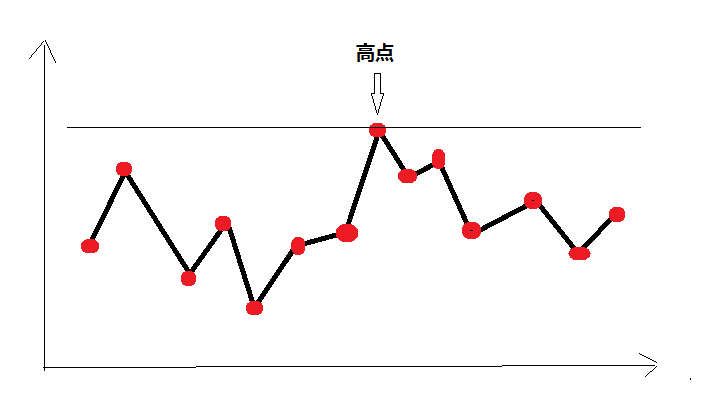
\includegraphics[width=0.8\textwidth]{img/2.png}%插入图片,按图片原尺寸插入
			\caption{高点的定义}
		\end{figure}
	
	\item 快速下跌的定义
	
	在回测中,我们定义了一类下跌:在相邻的两个高点之间的交易日中,如果存在某一个价格(只要在盘中出现即可)相比第一个高点的价格下跌了20\%以上,则认为这是一个快速下跌。通常在此类下跌过程中,反弹不超过两个周期。
	\item 反弹的定义:
	
	在回测中,我们定义了一类反弹:在出现快速下跌时,最低价格至第二个高点之间,认为是一段反弹。
	
	快速下跌和反弹如下图2所示。
		\begin{figure}[H]
			\centering
			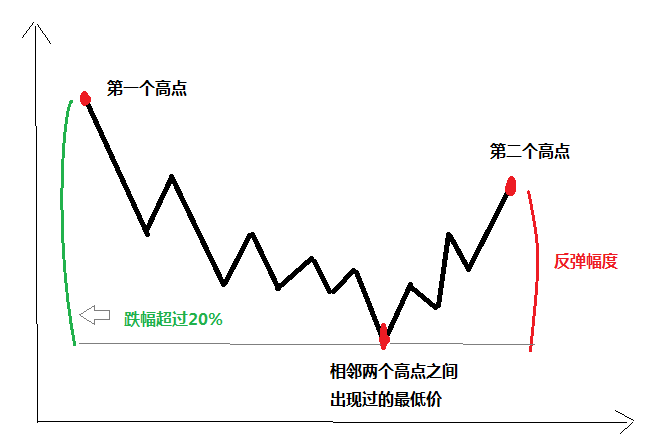
\includegraphics[width=0.8\textwidth]{img/3.png}%插入图片,按图片原尺寸插入
			\caption{高点的定义}
		\end{figure}

\end{itemize}



\subsection{回测结果}


\subsubsection{上证指数}
\begin{table}[H]
\centering  % 表居中
\begin{tabular}{|c|c|c|c|c|c|c|c|c|c|}  % {lccc} 表示各列元素对齐方式,left-l,right-r,center-c
\hline
高点一日期 & 点数 & 最低点日期 & 点数 & $\downarrow$ 天 &$\downarrow$幅度 & 高点二日期 & 点数 & $\uparrow$天& $\uparrow$ 幅度 \\ \hline
2005-04-13 & 1254 & 2005-06-06 & 998 & 33 & \textcolor{blue}{-20.4\%} & 2005-06-09 & 1146 & 3 & \textcolor{red}{14.8\%}  \\  \hline
2007-05-29 & 4335 & 2007-06-05 & 3404 & 5 & \textcolor{blue}{-21.5\%} & 2007-06-20 & 4311 & 11 & \textcolor{red}{26.7\%}  \\  \hline
2007-11-01 & 6005 & 2007-11-28 & 4778 & 19 & \textcolor{blue}{-20.4\%} & 2007-12-11 & 5209 & 9 & \textcolor{red}{9.0\%}  \\  \hline
2008-01-14 & 5522 & 2008-02-01 & 4195 & 14 & \textcolor{blue}{-24.0\%} & 2008-02-20 & 4695 & 8 & \textcolor{red}{11.9\%}  \\  \hline
2008-03-04 & 4472 & 2008-04-03 & 3271 & 22 & \textcolor{blue}{-26.9\%} & 2008-04-08 & 3656 & 2 & \textcolor{red}{11.8\%}  \\  \hline
2008-05-15 & 3706 & 2008-06-20 & 2695 & 25 & \textcolor{blue}{-27.3\%} & 2008-06-26 & 2931 & 4 & \textcolor{red}{8.7\%}  \\  \hline
2008-07-28 & 2924 & 2008-08-19 & 2284 & 16 & \textcolor{blue}{-21.9\%} & 2008-08-20 & 2523 & 1 & \textcolor{red}{10.5\%}  \\  \hline
2008-08-20 & 2523 & 2008-09-18 & 1802 & 20 & \textcolor{blue}{-28.6\%} & 2008-09-25 & 2333 & 5 & \textcolor{red}{29.5\%}  \\  \hline
2008-09-25 & 2333 & 2008-10-28 & 1664 & 18 & \textcolor{blue}{-28.6\%} & 2008-11-18 & 2050 & 15 & \textcolor{red}{23.2\%}  \\  \hline
2009-08-04 & 3478 & 2009-09-01 & 2639 & 20 & \textcolor{blue}{-24.1\%} & 2009-09-18 & 3068 & 13 & \textcolor{red}{16.2\%}  \\  \hline
2010-04-15 & 3181 & 2010-05-21 & 2481 & 25 & \textcolor{blue}{-22.0\%} & 2010-05-28 & 2686 & 5 & \textcolor{red}{8.2\%}  \\  \hline
2013-05-29 & 2334 & 2013-06-25 & 1849 & 16 & \textcolor{blue}{-20.8\%} & 2013-07-11 & 2092 & 12 & \textcolor{red}{13.1\%}  \\  \hline




\end{tabular}
\caption{2000年之后上证指数快速下跌后的反弹情况}
\end{table}

上证指数在下跌时,平均下跌时间为19.4个交易日,平均跌幅为 -23.8\%;平均反弹时间为7.3个交易日,平均反弹幅度为 15.3\%。


\subsubsection{恒生指数}

\begin{table}[H]
\centering  % 表居中
\begin{tabular}{|c|c|c|c|c|c|c|c|c|c|}  % {lccc} 表示各列元素对齐方式,left-l,right-r,center-c
\hline
高点一日期 & 点数 & 最低点日期 & 点数 & $\downarrow$ 天 &$\downarrow$幅度 & 高点二日期 & 点数 & $\uparrow$天& $\uparrow$ 幅度 \\ \hline
1992-11-12 & 6470 & 1992-12-03 & 4947 & 15 & \textcolor{blue}{-23.5\%} & 1992-12-16 & 5417 & 9 & \textcolor{red}{9.5\%}  \\  \hline
1994-02-04 & 12186 & 1994-03-22 & 8534 & 27 & \textcolor{blue}{-30.0\%} & 1994-04-13 & 9905 & 13 & \textcolor{red}{16.1\%}  \\  \hline
1994-11-17 & 9620 & 1994-12-12 & 7670 & 17 & \textcolor{blue}{-20.3\%} & 1994-12-22 & 8460 & 8 & \textcolor{red}{10.3\%}  \\  \hline
1997-08-07 & 16820 & 1997-09-02 & 12899 & 17 & \textcolor{blue}{-23.3\%} & 1997-09-09 & 15043 & 5 & \textcolor{red}{16.6\%}  \\  \hline
1997-10-06 & 15242 & 1997-10-28 & 8775 & 15 & \textcolor{blue}{-42.4\%} & 1997-11-04 & 11661 & 5 & \textcolor{red}{32.9\%}  \\  \hline
1997-12-31 & 10935 & 1998-01-12 & 7909 & 6 & \textcolor{blue}{-27.7\%} & 1998-02-11 & 11189 & 12 & \textcolor{red}{41.5\%}  \\  \hline
1998-05-21 & 9725 & 1998-06-16 & 7351 & 18 & \textcolor{blue}{-24.4\%} & 1998-07-02 & 8970 & 11 & \textcolor{red}{22.0\%}  \\  \hline
1998-07-17 & 8712 & 1998-08-13 & 6544 & 19 & \textcolor{blue}{-24.9\%} & 1998-08-27 & 7926 & 9 & \textcolor{red}{21.1\%}  \\  \hline
2000-03-28 & 18397 & 2000-05-12 & 14288 & 24 & \textcolor{blue}{-22.3\%} & 2000-05-17 & 15293 & 3 & \textcolor{red}{7.0\%}  \\  \hline
2001-02-07 & 16060 & 2001-04-09 & 12061 & 42 & \textcolor{blue}{-24.9\%} & 2001-04-19 & 13621 & 6 & \textcolor{red}{12.9\%}  \\  \hline
2001-08-16 & 12195 & 2001-09-21 & 8894 & 26 & \textcolor{blue}{-27.1\%} & 2001-10-11 & 10638 & 9 & \textcolor{red}{19.6\%}  \\  \hline
2007-12-27 & 28343 & 2008-01-22 & 21709 & 16 & \textcolor{blue}{-23.4\%} & 2008-02-04 & 25101 & 9 & \textcolor{red}{15.6\%}  \\  \hline
2008-08-28 & 21546 & 2008-09-18 & 16283 & 14 & \textcolor{blue}{-24.4\%} & 2008-09-22 & 19869 & 2 & \textcolor{red}{22.0\%}  \\  \hline
2008-09-22 & 19869 & 2008-10-27 & 10676 & 19 & \textcolor{blue}{-46.3\%} & 2008-11-05 & 15317 & 7 & \textcolor{red}{43.5\%}  \\  \hline
2008-11-05 & 15317 & 2008-11-21 & 11814 & 12 & \textcolor{blue}{-22.9\%} & 2008-12-11 & 15781 & 14 & \textcolor{red}{33.6\%}  \\  \hline
2009-01-07 & 15763 & 2009-01-21 & 12439 & 10 & \textcolor{blue}{-21.1\%} & 2009-02-10 & 13976 & 9 & \textcolor{red}{12.4\%}  \\  \hline


\end{tabular}
\caption{1991年之后恒生指数快速下跌后的反弹情况}
\end{table}

恒生指数在下跌时,平均下跌时间为18.8个交易日,平均跌幅为 -26.8\%;平均反弹时间为8.2个交易日,平均反弹幅度为 21.0\%。

\subsubsection{标普500}


\begin{table}[H]
\centering  % 表居中
\begin{tabular}{|c|c|c|c|c|c|c|c|c|c|}  % {lccc} 表示各列元素对齐方式,left-l,right-r,center-c
\hline

高点一日期 & 点数 & 最低点日期 & 点数 & $\downarrow$ 天 &$\downarrow$幅度 & 高点二日期 & 点数 & $\uparrow$天& $\uparrow$幅度 \\ \hline
2001-02-06 & 1363 & 2001-03-22 & 1081 & 31 & \textcolor{blue}{-20.7\%} & 2001-03-27 & 1183 & 3 & \textcolor{red}{9.4\%}  \\  \hline
2001-08-27 & 1186 & 2001-09-21 & 944 & 14 & \textcolor{blue}{-20.4\%} & 2001-10-17 & 1107 & 13 & \textcolor{red}{17.2\%}  \\  \hline
2002-06-18 & 1040 & 2002-07-24 & 775 & 25 & \textcolor{blue}{-25.5\%} & 2002-07-31 & 911 & 5 & \textcolor{red}{17.5\%}  \\  \hline
2008-09-19 & 1265 & 2008-10-10 & 839 & 10 & \textcolor{blue}{-33.6\%} & 2008-11-04 & 1007 & 17 & \textcolor{red}{20.0\%}  \\  \hline
2008-11-04 & 1007 & 2008-11-21 & 741 & 13 & \textcolor{blue}{-26.5\%} & 2008-11-28 & 896 & 4 & \textcolor{red}{20.9\%}  \\  \hline
2009-02-09 & 875 & 2009-03-06 & 666 & 18 & \textcolor{blue}{-23.8\%} & 2009-04-17 & 875 & 28 & \textcolor{red}{31.3\%}  \\  \hline



\end{tabular}
\caption{1991年之后标普500指数快速下跌后的反弹情况}
\end{table}

标普500指数在下跌时,平均下跌时间为18.5个交易日,平均跌幅为 -25.1\%;平均反弹时间为11.6个交易日,平均反弹幅度为 19.4\%。

\subsection{三个指数比较}

根据前面的结果可知:


\begin{table}[H]
\centering  % 表居中
\begin{tabular}{|c|c|c|c|}  % {lccc} 表示各列元素对齐方式,left-l,right-r,center-c
\hline
& 上证指数 & 恒生指数 & 标普500 \\ \hline 
出现次数& 12 & 16 & 6 \\ \hline
平均下跌时间 & 19.4 & 18.8 & 18.5 \\ \hline
平均下跌幅度 & \textcolor{blue}{-23.8\%}  & \textcolor{blue}{-26.8\%}  &\textcolor{blue}{-25.1\%}  \\ \hline
平均反弹时间 & 7.3   & 8.2 & 11.6 \\ \hline
平均反弹幅度 & \textcolor{red}{15.3\%}  & \textcolor{red}{21.0 \%}  & \textcolor{red}{19.4 \%}  \\ \hline


\end{tabular}
\caption{三大指数的数据比较}
\end{table}


\subsection{下跌原因分析}

\subsubsection{上证指数}
注:下文中贴有K线图,放在大屏显示器上看效果会好一些。

\begin{enumerate}[1)]

\item 2005-04-13 $\sim$ 2005-06-09
	
	 2005年5月,管理层启动股改试点,2005年6月6日证监会推出《上市公司回购社会公众股份管理办法(试行)》。
	 
	 
	 \begin{figure}[H]
		\centering
		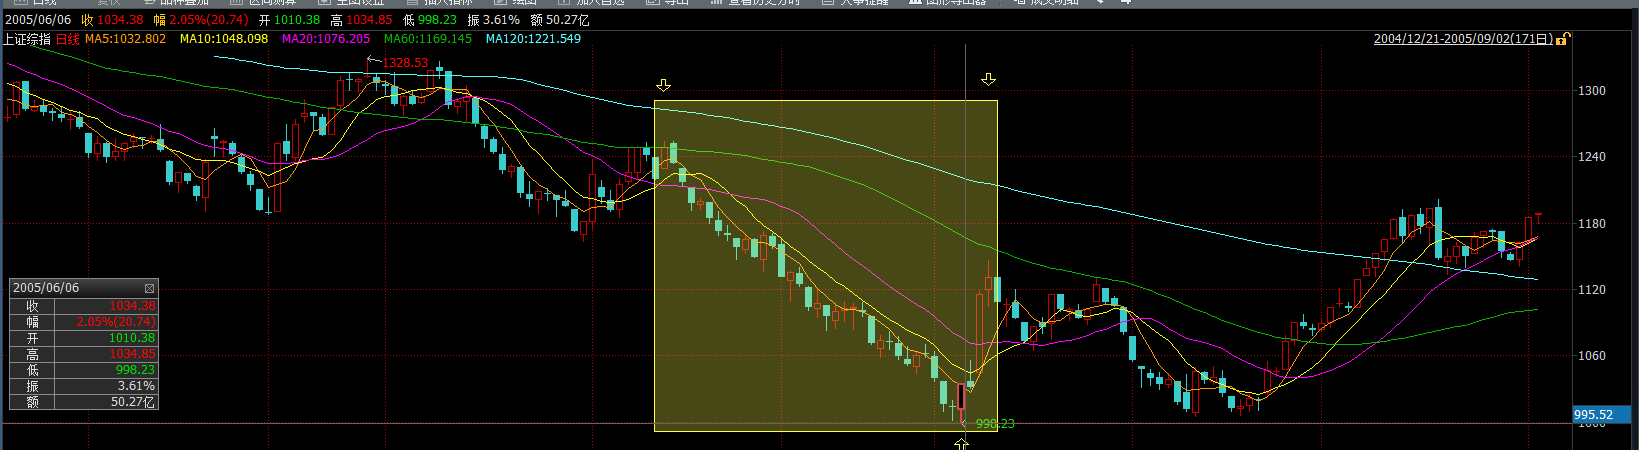
\includegraphics[width=0.9\textwidth]{img/11.png}%插入图片,按图片原尺寸插入
		\caption{上证指数K线图1}
	\end{figure}
		
	上图是2004年4月\~2006年4月的日K线图。由图可以看出,2005年4月\~2005年6月处于下跌通道中,2005年6月6日的最低点是全年的最低点,之后开启了一波新的上涨行情。
\item 2007-05-29 $\sim$2007-06-20
	
	“530”印花税上调。
	
	 \begin{figure}[H]
		\centering
		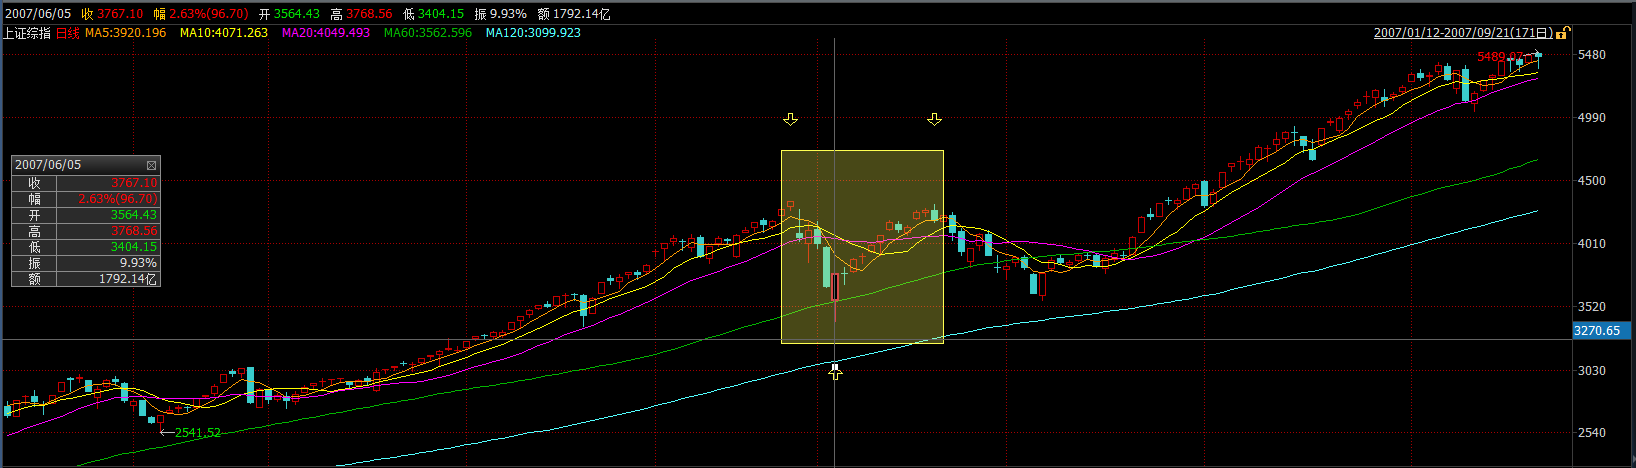
\includegraphics[width=0.9\textwidth]{img/12.png}%插入图片,按图片原尺寸插入
		\caption{上证指数K线图2}
	\end{figure}
	
	
	
\item 2007-11-01 $\sim$ 2007-12-11 

	2007年10月中石油上市,指数到达6124大顶,11月份有一波小回调。之后结束了牛市,开启了下跌行情。

	\begin{figure}[H]
		\centering
		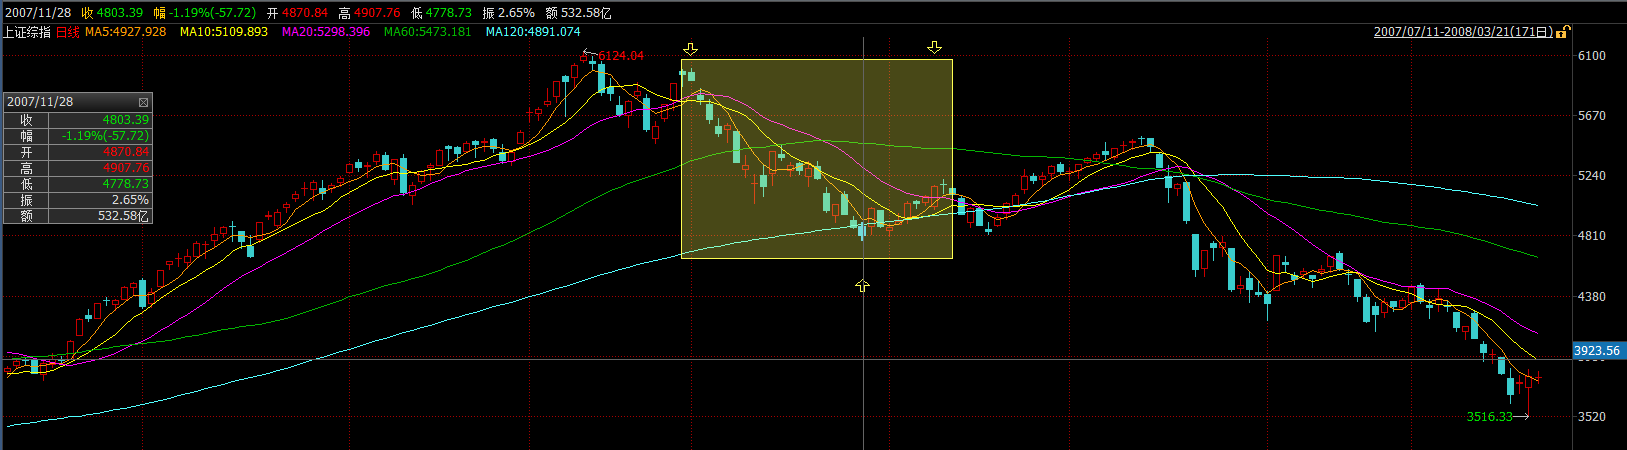
\includegraphics[width=0.9\textwidth]{img/13.png}%插入图片,按图片原尺寸插入
		\caption{上证指数K线图3}
	\end{figure}
	
\item 2008-01-14 $\sim$ 2008-02-20

2008年1月16日,中国人民银行宣布自1月25日起上调存款类金融机构人民币存款准备金率0.5个百分点。至此,存款准备金率上调至15\%,此属当时历史高位。

	\begin{figure}[H]
		\centering
		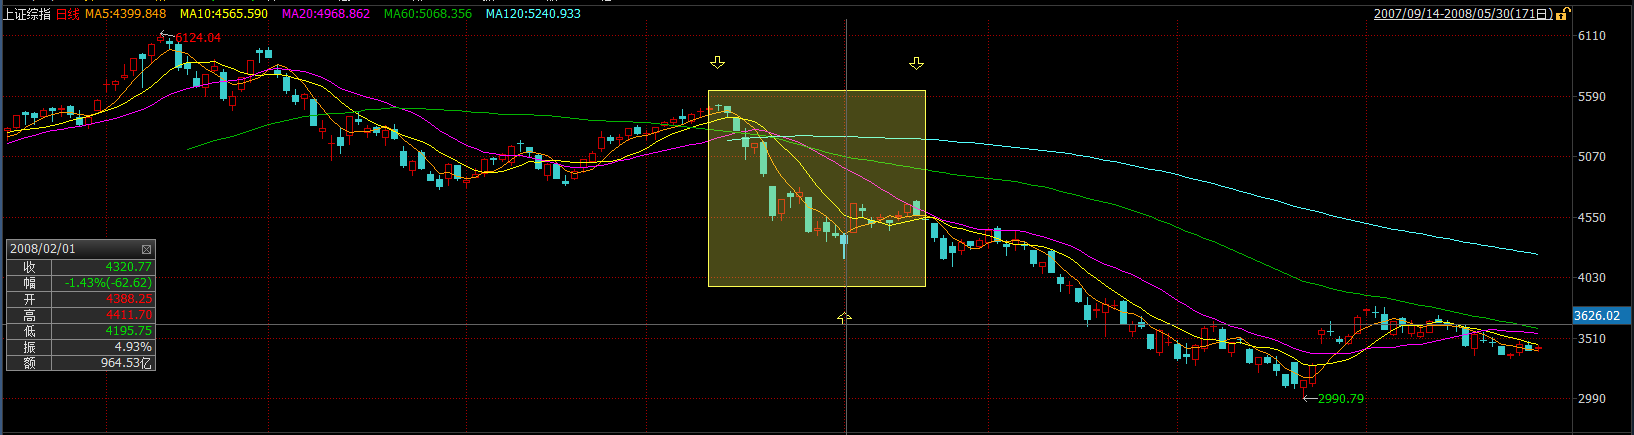
\includegraphics[width=0.9\textwidth]{img/14.png}%插入图片,按图片原尺寸插入
		\caption{上证指数K线图4}
	\end{figure}
	
\item 2008-03-04 $\sim$ 2008-04-08

	\begin{figure}[H]
		\centering
		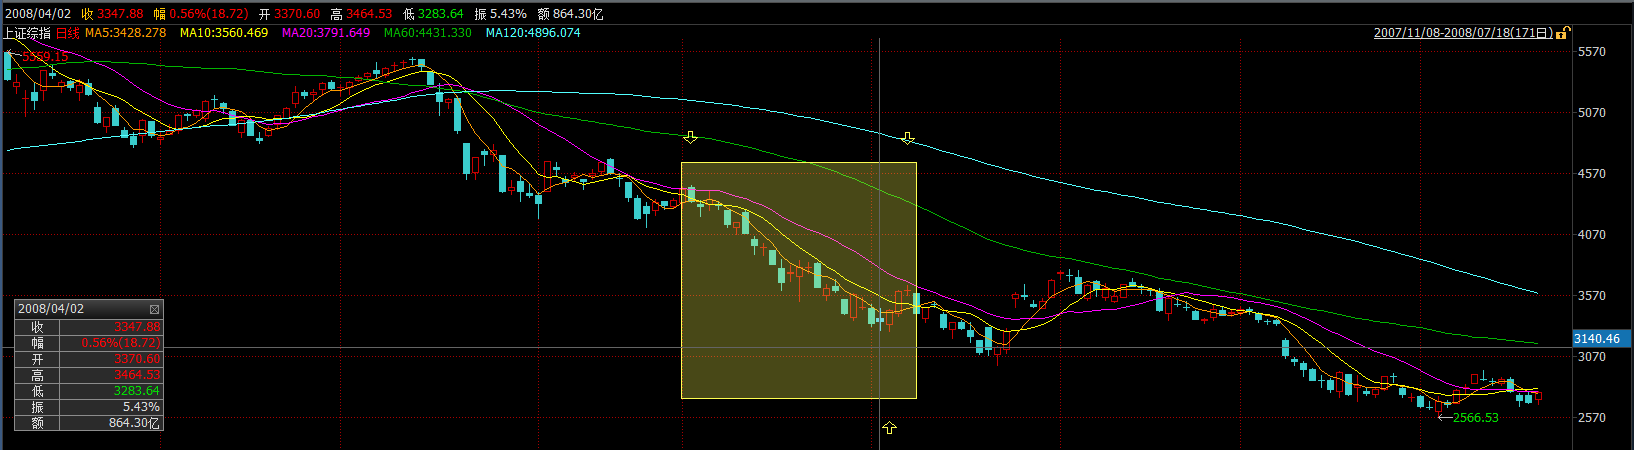
\includegraphics[width=0.9\textwidth]{img/15.png}%插入图片,按图片原尺寸插入
		\caption{上证指数K线图5}
	\end{figure}

\item 2008-05-15 $\sim$ 2008-06-26 
	\begin{itemize}
		\item 在5月CPI数据尚未公布前,央行上调存款准备金率1个百分点,释放“从紧”强烈信号;
		\item   国际油价一日暴涨10美元创新高,全球股市震荡加剧;
		\item 中国建筑和陕西天然气的首发申请成功过会,A股面临扩容压力。
	
	\end{itemize}
	

	\begin{figure}[H]
		\centering
		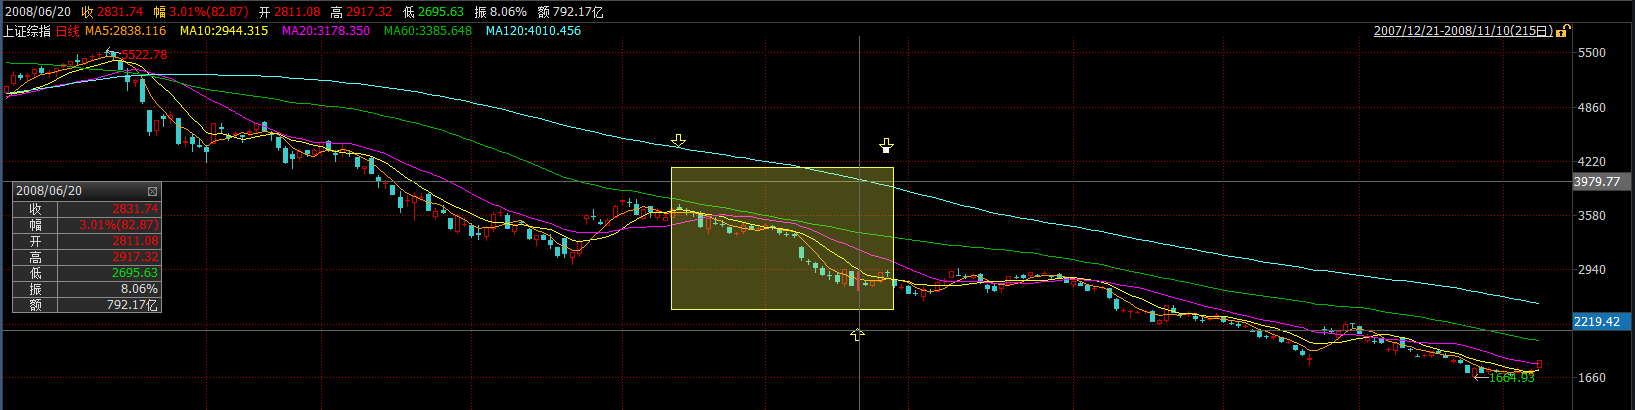
\includegraphics[width=0.9\textwidth]{img/16.png}%插入图片,按图片原尺寸插入
		\caption{上证指数K线图6}
	\end{figure}

\item 2008-07-28 $\sim$ 2008-08-20

	\begin{figure}[H]
		\centering
		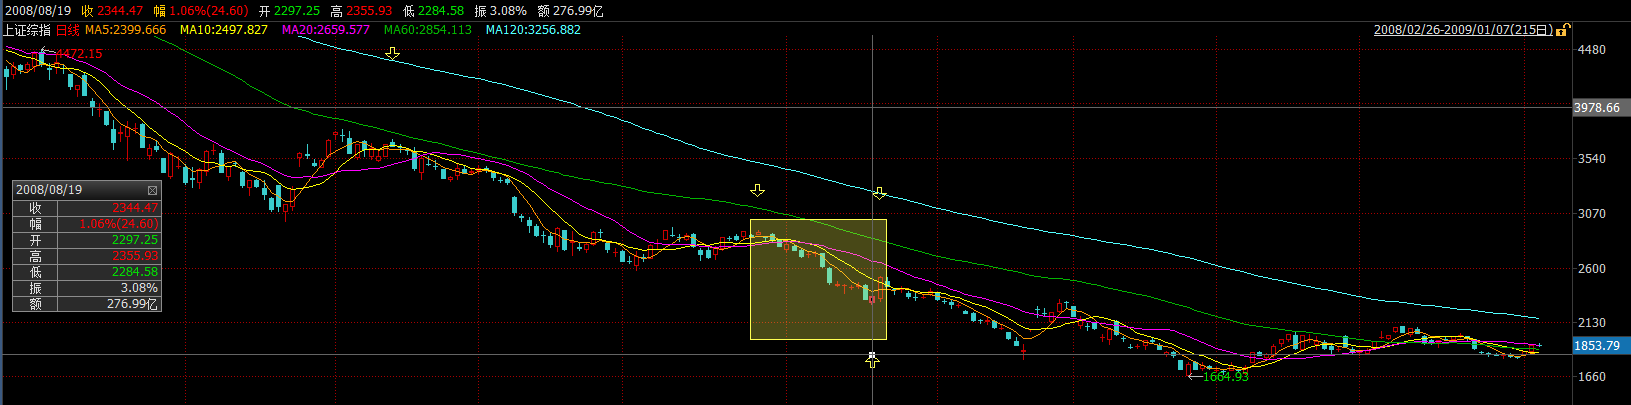
\includegraphics[width=0.9\textwidth]{img/17.png}%插入图片,按图片原尺寸插入
		\caption{上证指数K线图7}
	\end{figure}
	
\item 2008-08-20 $\sim$ 2008-09-25

9月19日,沪指收盘报2075点,涨179点,涨幅9.46\%,深成指收盘报7154点,涨590.94点,涨幅9\%,个股几乎全线涨停。
	\begin{itemize}
	\item 印花税单边征收;
	\item 汇金公司增持工、中、建三大银行股份;
	\item 国资委支持央企增持或回收上市公司股份三大举措出台
	
	\end{itemize}

	\begin{figure}[H]
		\centering
		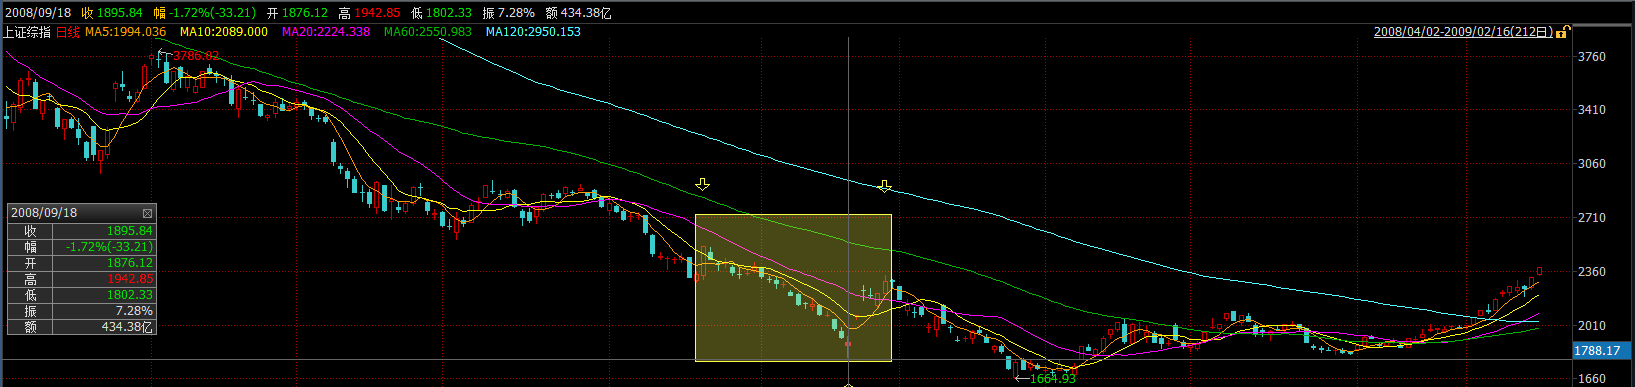
\includegraphics[width=0.9\textwidth]{img/18.png}%插入图片,按图片原尺寸插入
		\caption{上证指数K线图8}
	\end{figure}	

\item 2008-09-25 $\sim$ 2008-11-18

10月28日创下了近三年低点——1664.93

	\begin{itemize}
	\item 印花税单边征收;
	\item 汇金公司增持工、中、建三大银行股份;
	\item 国资委支持央企增持或回收上市公司股份三大举措出台
	
	\end{itemize}

	\begin{figure}[H]
		\centering
		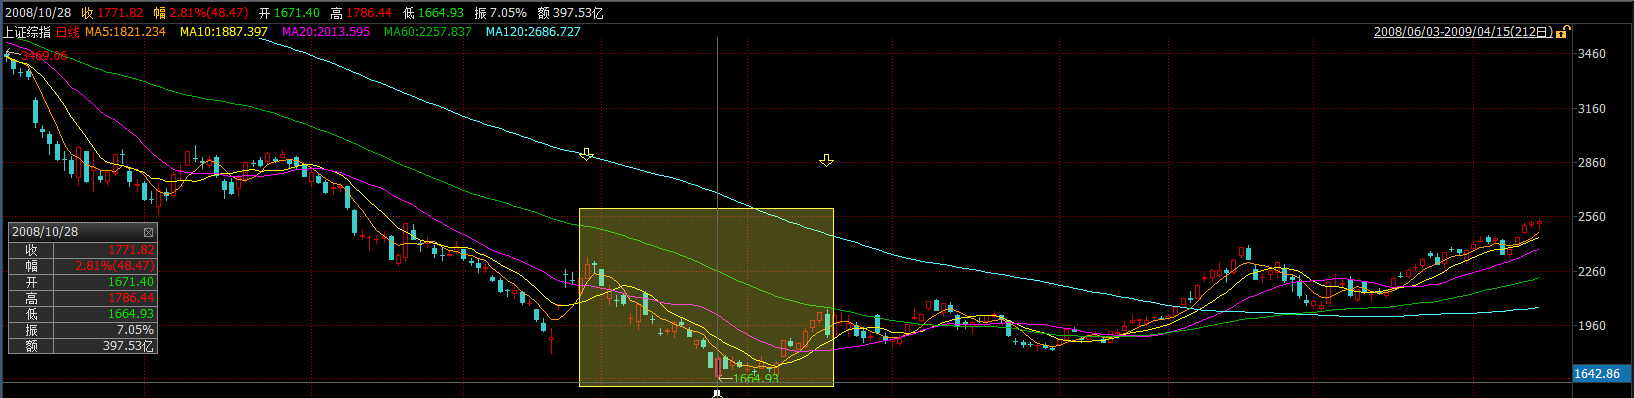
\includegraphics[width=0.9\textwidth]{img/19.png}%插入图片,按图片原尺寸插入
		\caption{上证指数K线图9}
	\end{figure}	

\item 2009-08-04 $\sim$ 2009-09-18

到达3478的高点后的第一个回调。

	\begin{figure}[H]
		\centering
		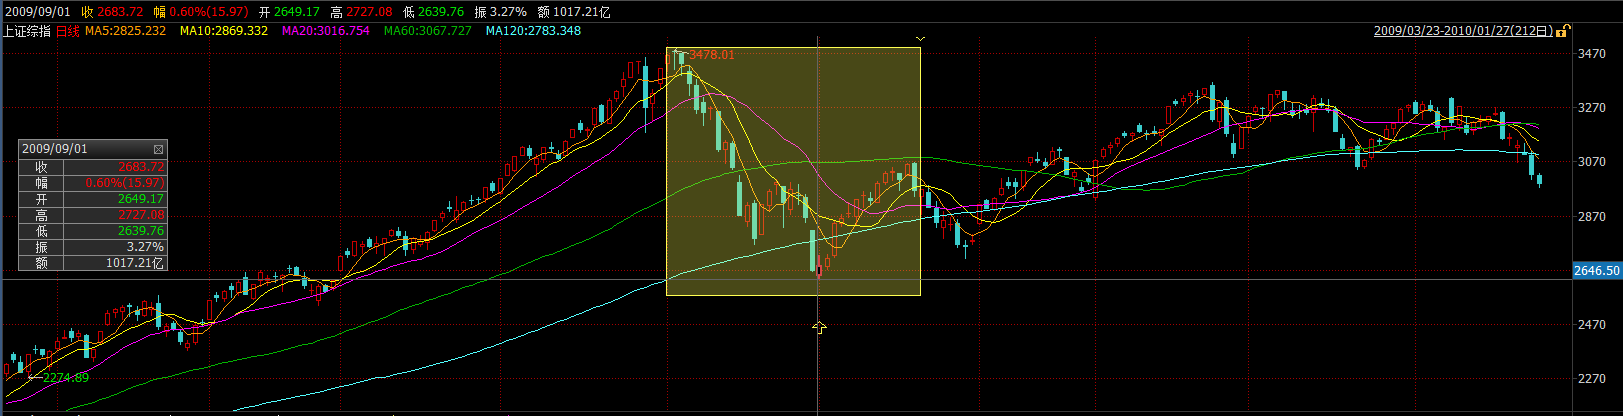
\includegraphics[width=0.9\textwidth]{img/20.png}%插入图片,按图片原尺寸插入
		\caption{上证指数K线图10}
	\end{figure}	

\item 2010-04-15 $\sim$ 2010-05-28
	\begin{itemize}
		\item 2010年5月,欧洲主权债务危机再次引发了全球金融市场慌乱,欧美股市表现低迷,各主要股指纷纷大幅下滑,道琼斯工业指数下跌7.9\%,标准普尔指数下跌8.2\%,英国富时100指数和日经指数分别下滑6.6\%和11.7\%。香港股市呈现先抑后扬走势,但受周边市场拖累,月内下跌6.36\%。
		\item A股市场多空交织,走势震荡下行,上证综指和深成指分别大跌9.7\%和8.59\%。
		\item 受政策前景不确定性的影响,中资银行股价继续承压。
	
	\end{itemize}


	\begin{figure}[H]
		\centering
		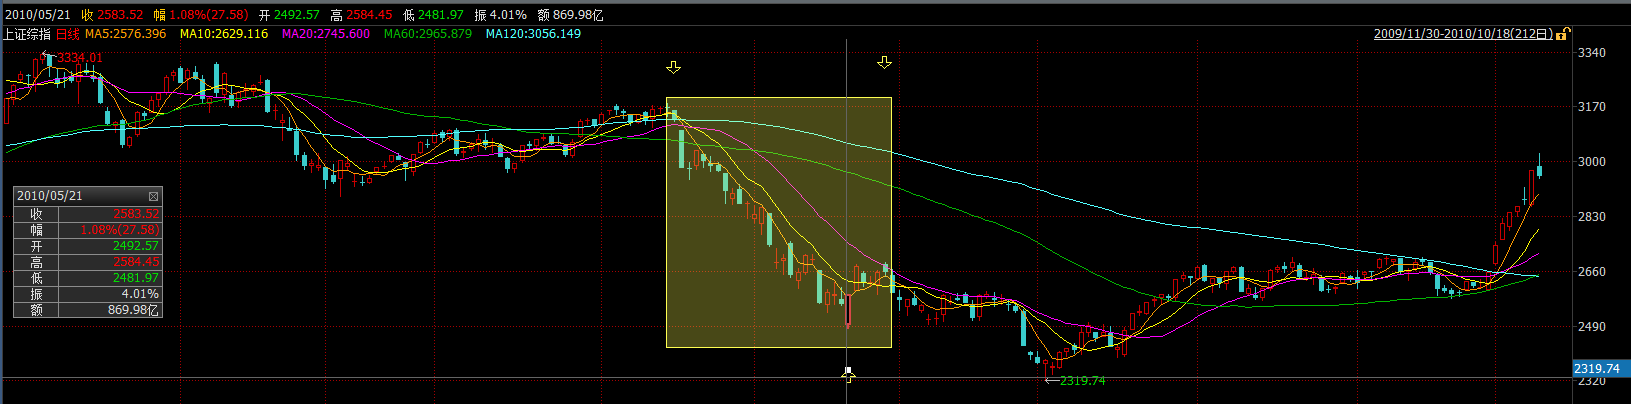
\includegraphics[width=0.9\textwidth]{img/21.png}%插入图片,按图片原尺寸插入
		\caption{上证指数K线图11}
	\end{figure}	

\item 2013-05-29 $\sim$ 2013-07-11 
	
	“624”暴跌
		
	\begin{itemize}
		\item  证监会否认了IPO将于7月底开闸,并表示IPO开闸无时间表。市场面临巨大的不确定性。\item 有分析称“钱荒”或闹到7月中旬,而中央对此罕见地“袖手旁观”,且6月底有1.5万亿人民币理财产品到期,流动性第二波冲击即将降临,股市承压。
		\item 据测算上周基金平均仓位降至77.39\%,与前一周相比下降了1.26个百分点,大跌中基金主力砸盘推波助澜。
		\item 伯南克明确未来将退出QE,外围股市一片哀鸿,全球市场多头一败涂地,A股外忧内患
	
	\end{itemize}
	\begin{figure}[H]
		\centering
		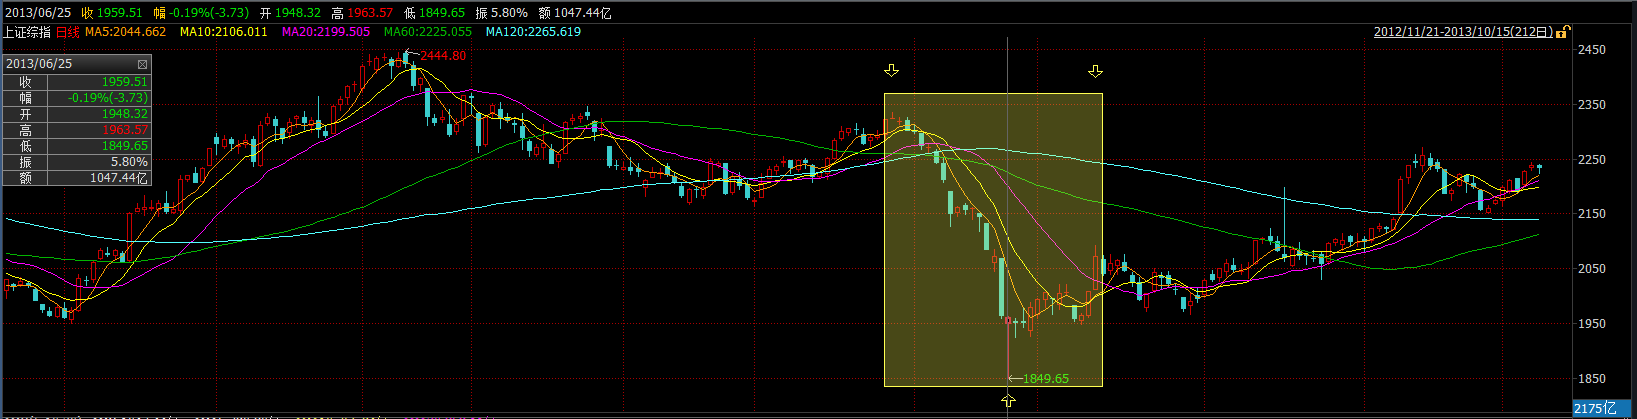
\includegraphics[width=0.9\textwidth]{img/22.png}%插入图片,按图片原尺寸插入
		\caption{上证指数K线图12}
	\end{figure}	
	
\end{enumerate}

\subsubsection{恒生指数}

\begin{enumerate}
	\item 1992-11-12 $\sim$ 1992-12-16
	
	上涨过程中的回调,4个月后又突破新高。香港在90年代转口贸易和金融业不断增强,成为逐渐崛起的金融中心。
	
	\begin{figure}[H]
		\centering
		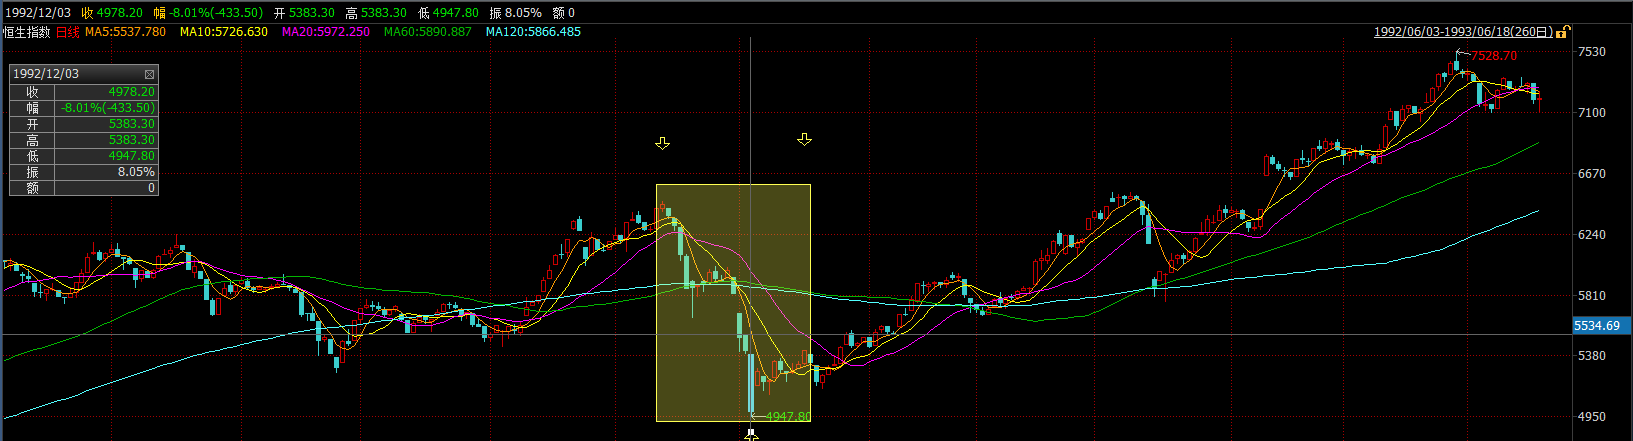
\includegraphics[width=0.9\textwidth]{img/31.png}%插入图片,按图片原尺寸插入
		\caption{恒生指数K线图1}
	\end{figure}	
	
	\item 1994-02-04 $\sim$ 1994-04-13
	
	恒生指数在1994年2月4日达到12157点,之后经历了一段时期的下调。1994年$\sim$1995年总体趋势是:外资撤离,中资入场,动荡中的下跌。
	
	\begin{figure}[H]
		\centering
		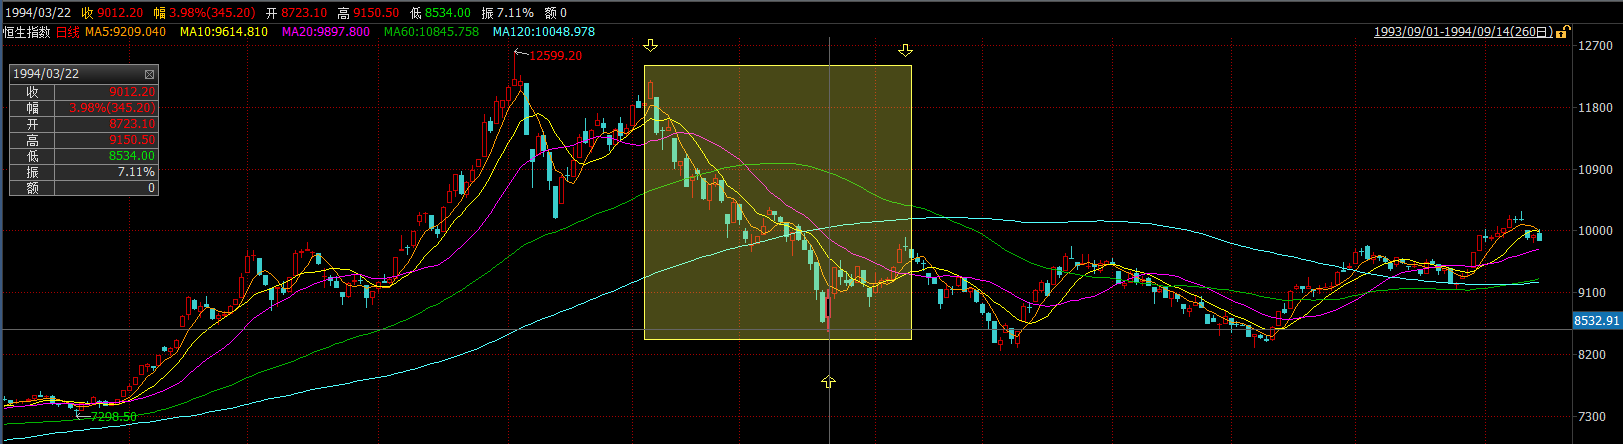
\includegraphics[width=0.9\textwidth]{img/32.png}%插入图片,按图片原尺寸插入
		\caption{恒生指数K线图2}
	\end{figure}	
	
	\item 1994-11-17 $\sim$ 1994-12-22
	
	\begin{figure}[H]
		\centering
		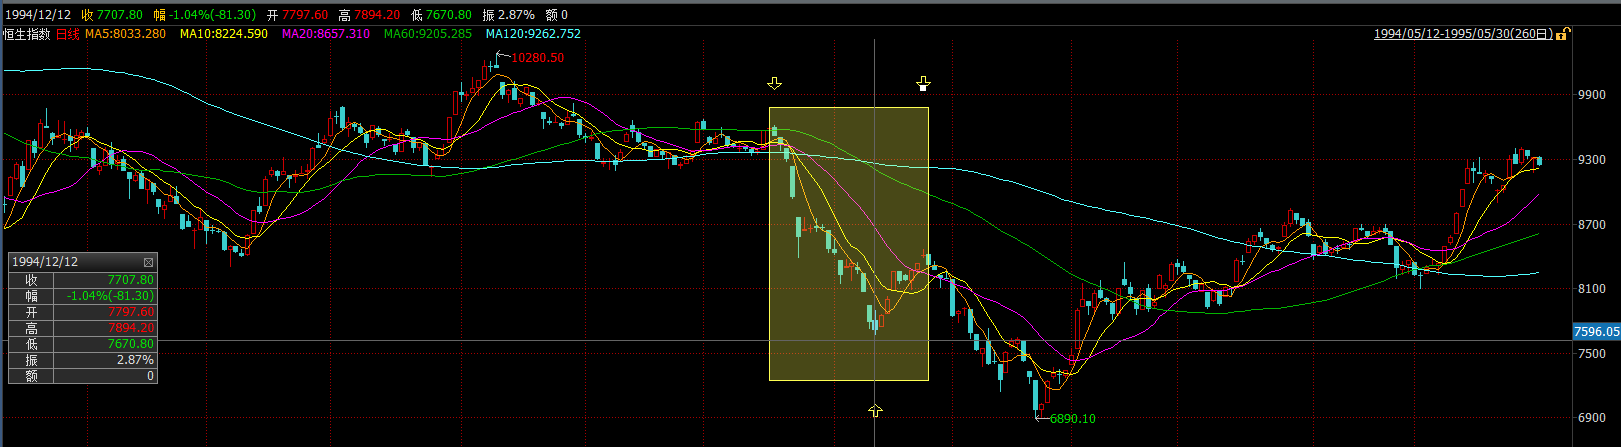
\includegraphics[width=0.9\textwidth]{img/33.png}%插入图片,按图片原尺寸插入
		\caption{恒生指数K线图3}
	\end{figure}	
		
	\item 1997-08-07 $\sim$ 1997-09-09
	
	东南亚金融危机
	
		\begin{figure}[H]
		\centering
		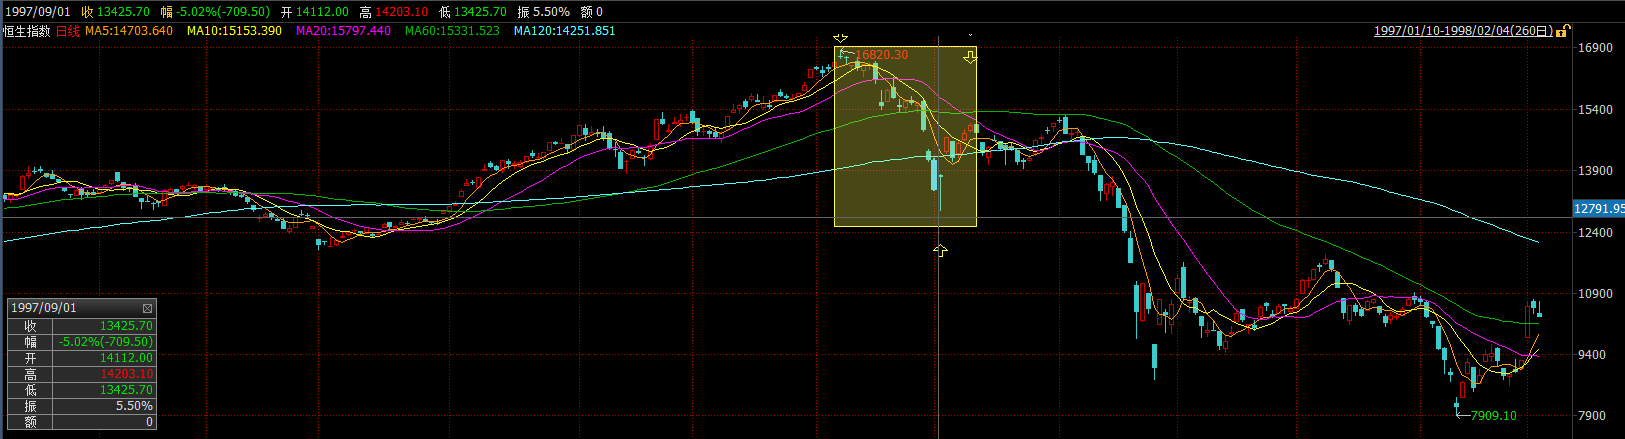
\includegraphics[width=0.9\textwidth]{img/34.png}%插入图片,按图片原尺寸插入
		\caption{恒生指数K线图4}
	\end{figure}	
	
	\item 1997-10-06 $\sim$ 1997-11-04
	
	东南亚金融危机
		\begin{figure}[H]
		\centering
		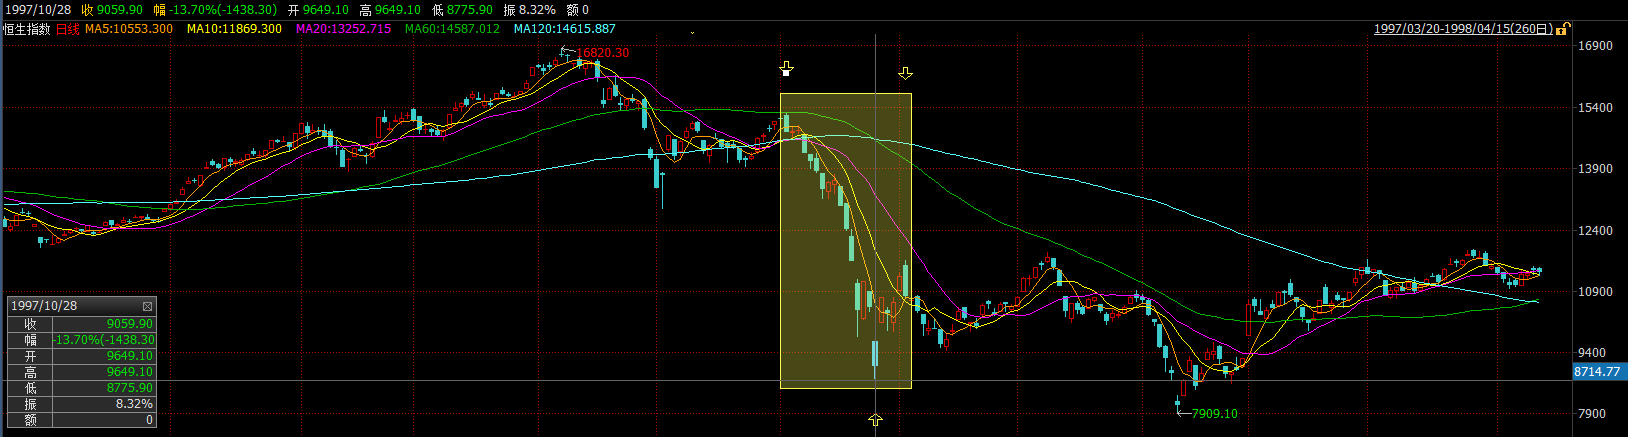
\includegraphics[width=0.9\textwidth]{img/35.png}%插入图片,按图片原尺寸插入
		\caption{恒生指数K线图5}
	\end{figure}	
	
	\item 1997-12-31 $\sim$ 1998-02-11
	
	东南亚金融危机
		\begin{figure}[H]
		\centering
		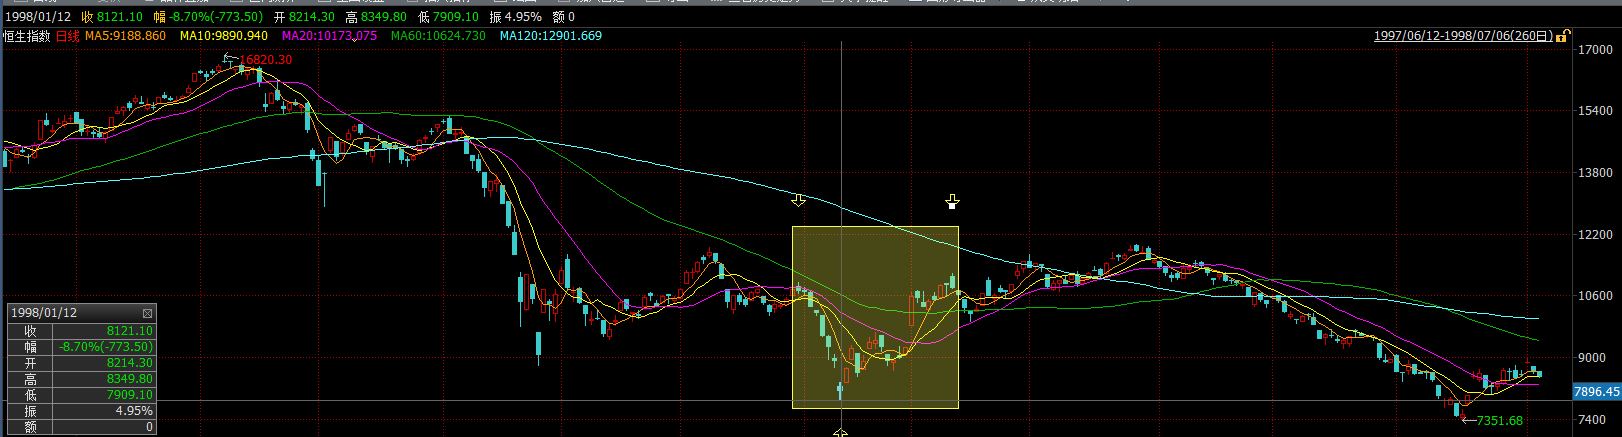
\includegraphics[width=0.9\textwidth]{img/36.png}%插入图片,按图片原尺寸插入
		\caption{恒生指数K线图6}
	\end{figure}	
	
	\item 1998-05-21 $\sim$ 1998-07-02
	
	东南亚金融危机
		\begin{figure}[H]
		\centering
		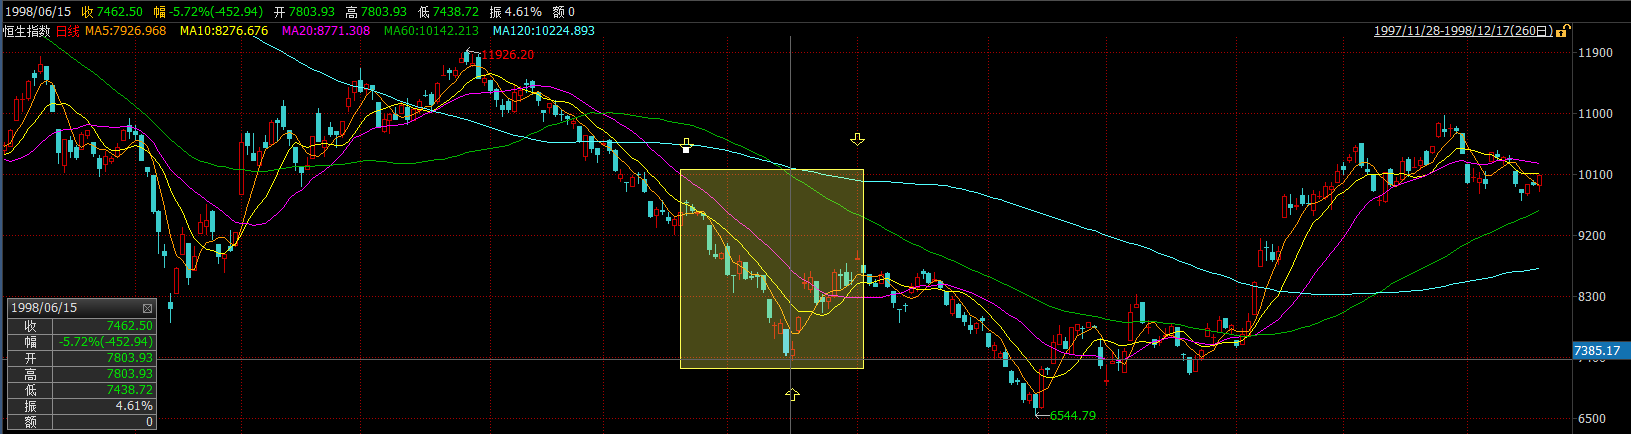
\includegraphics[width=0.9\textwidth]{img/37.png}%插入图片,按图片原尺寸插入
		\caption{恒生指数K线图7}
	\end{figure}	
	
	\item 1998-07-17 $\sim$ 1998-08-27 
	
	东南亚金融危机
		\begin{figure}[H]
		\centering
		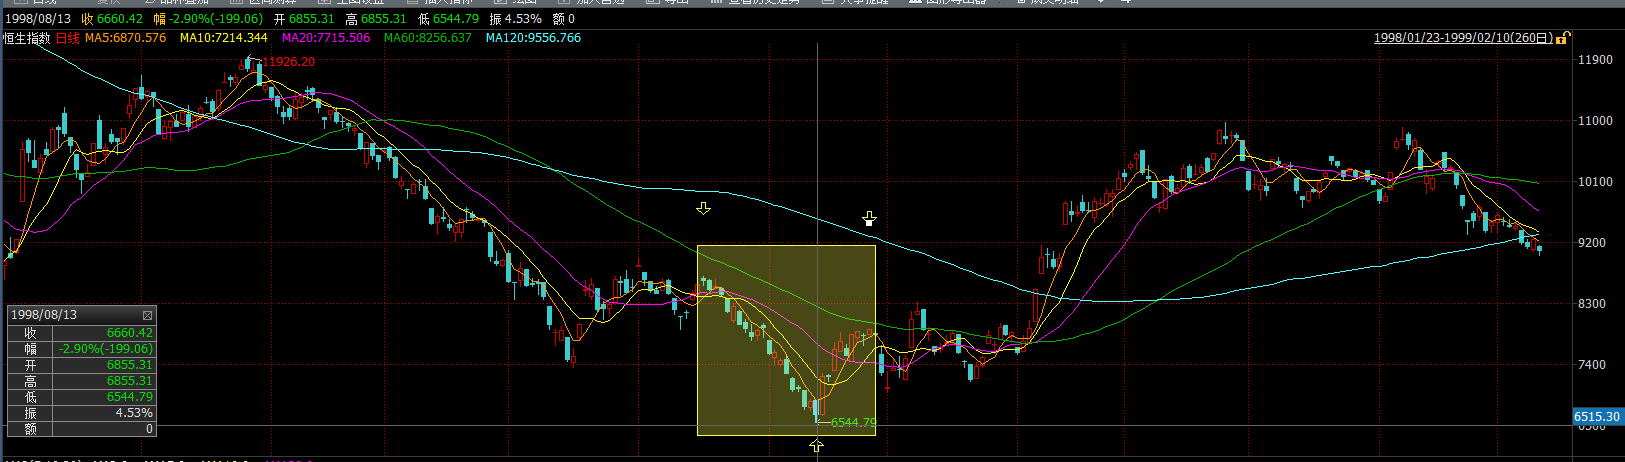
\includegraphics[width=0.9\textwidth]{img/38.png}%插入图片,按图片原尺寸插入
		\caption{恒生指数K线图8}
	\end{figure}		
	
	\item 2000-03-28 $\sim$ 2000-05-17
	
	在2000年3月28日达到18397点的高点,相比一年前涨幅超过100\%,这是初次回调
	
	\begin{figure}[H]
		\centering
		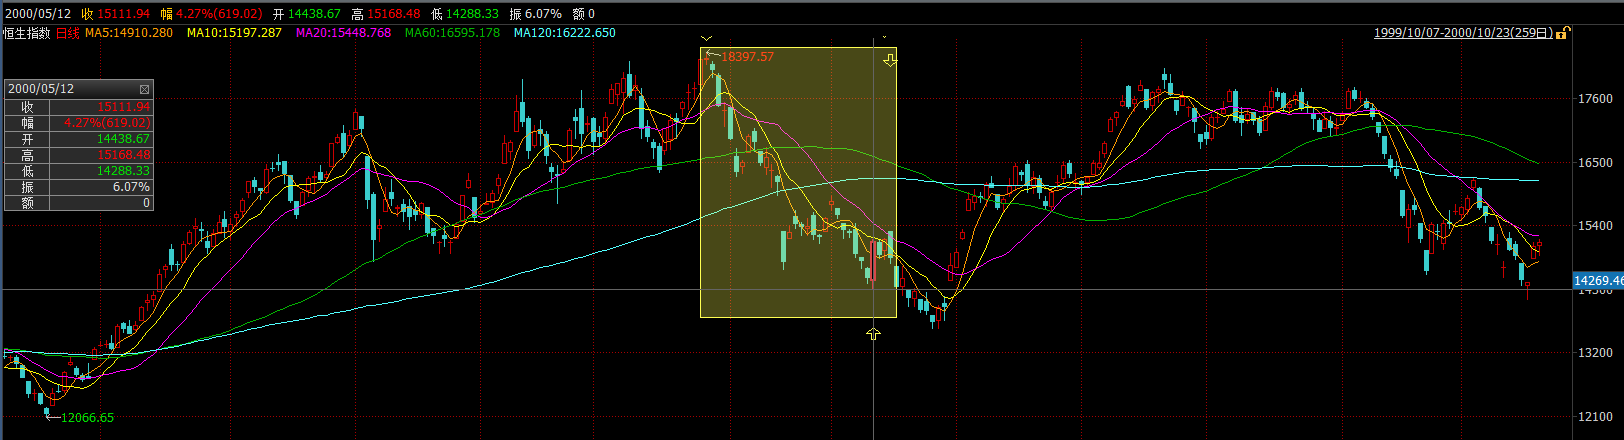
\includegraphics[width=0.9\textwidth]{img/39.png}%插入图片,按图片原尺寸插入
		\caption{恒生指数K线图9}
	\end{figure}	
	
	\item 2001-02-07 $\sim$ 2001-04-19
	
	互联网泡沫破灭,处于下跌趋势中。
		\begin{figure}[H]
		\centering
		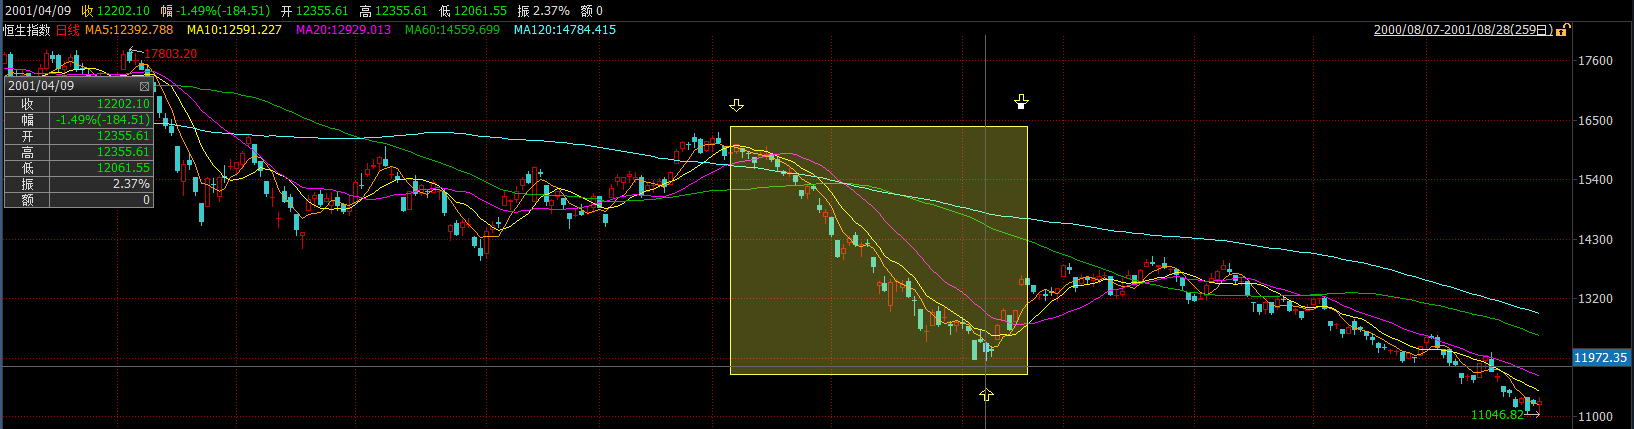
\includegraphics[width=0.9\textwidth]{img/40.png}%插入图片,按图片原尺寸插入
		\caption{恒生指数K线图10}
	\end{figure}
	
	\item 2001-08-16 $\sim$ 2001-10-11
		
	互联网泡沫破灭,处于下跌趋势中。

	\begin{figure}[H]
		\centering
		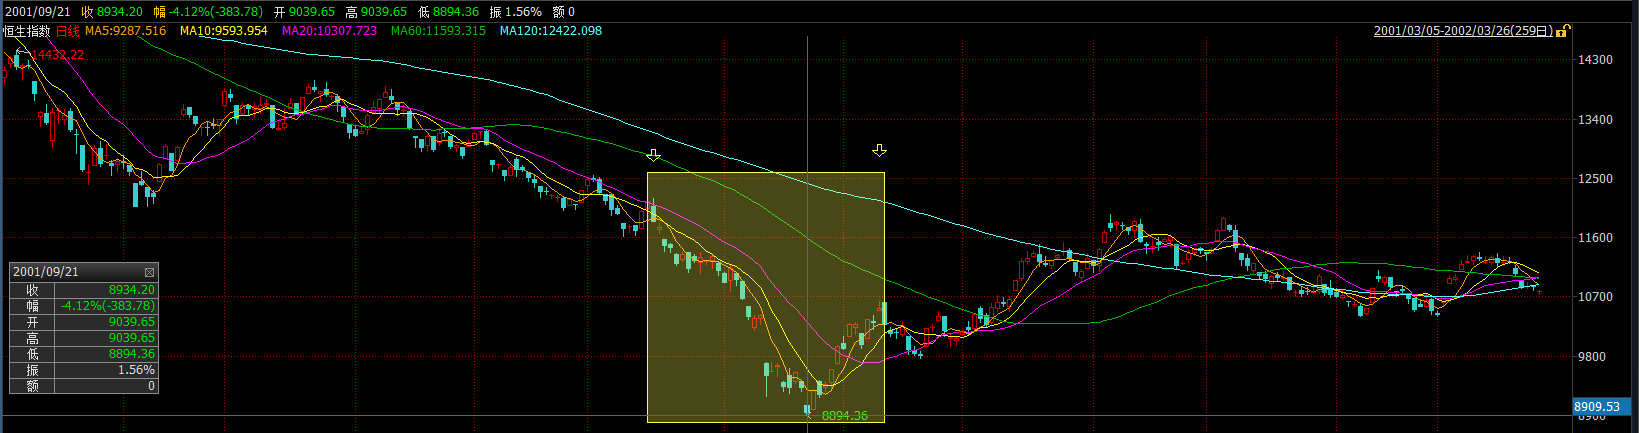
\includegraphics[width=0.9\textwidth]{img/41.png}%插入图片,按图片原尺寸插入
		\caption{恒生指数K线图11}
	\end{figure}
	
	\item 2007-12-27 $\sim$ 2008-02-04
	
	全球金融危机
	
	\begin{figure}[H]
		\centering
		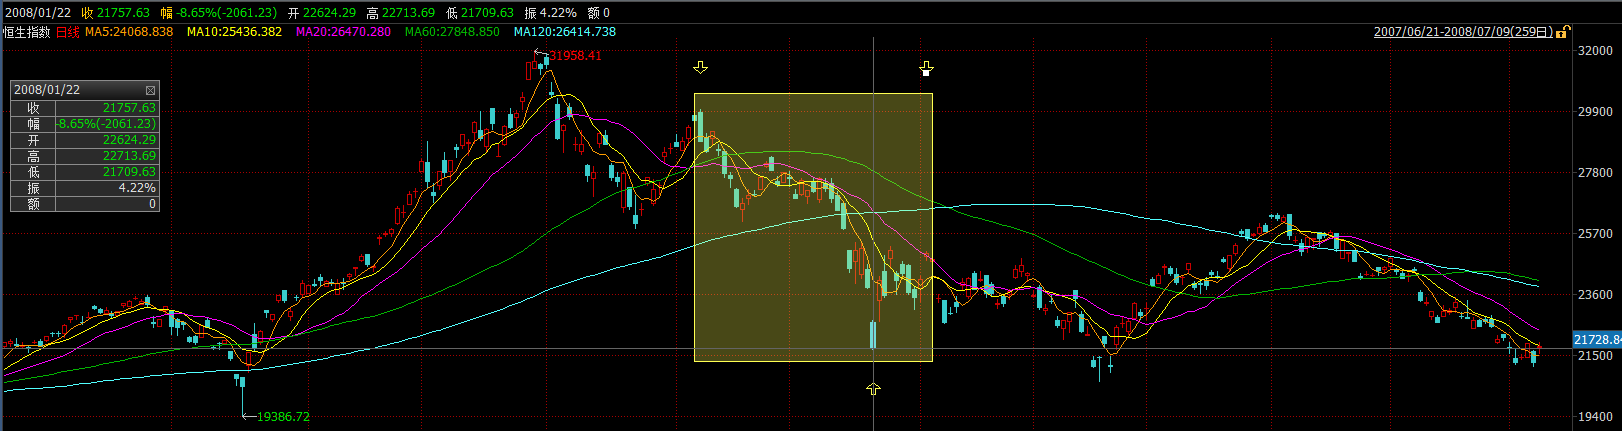
\includegraphics[width=0.9\textwidth]{img/42.png}%插入图片,按图片原尺寸插入
		\caption{恒生指数K线图12}
	\end{figure}
	
	\item 2008-08-28 $\sim$ 2008-09-22
	
	下跌通道中
	
	\begin{figure}[H]
		\centering
		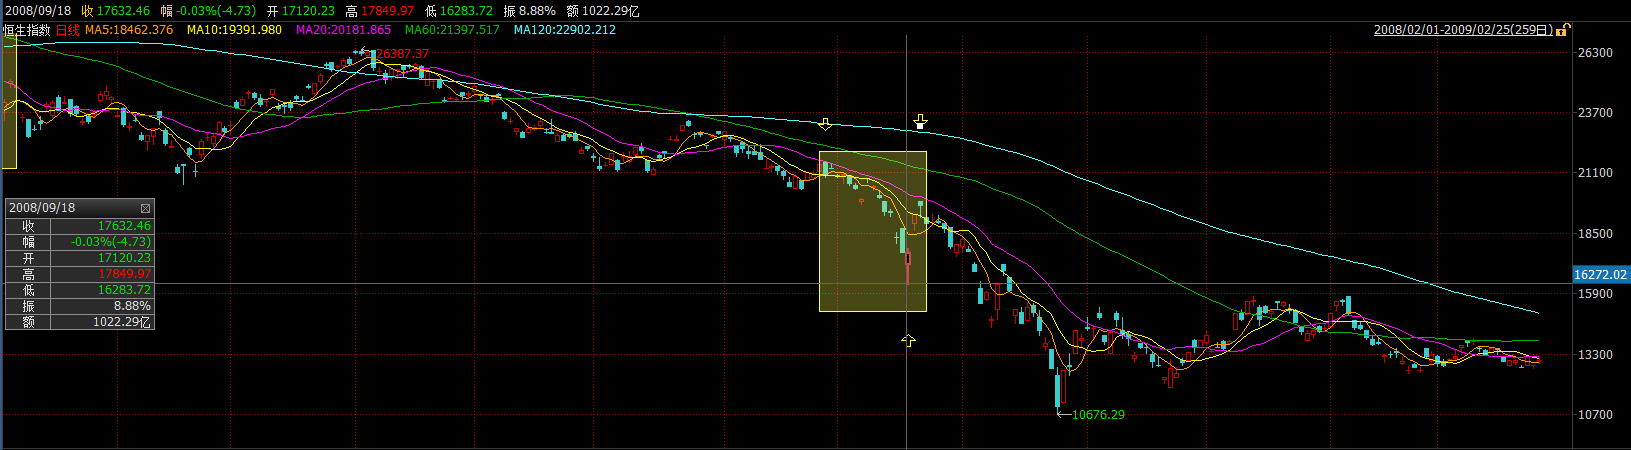
\includegraphics[width=0.9\textwidth]{img/43.png}%插入图片,按图片原尺寸插入
		\caption{恒生指数K线图13}
	\end{figure}
	
	
	\item 2008-09-22 $\sim$ 2008-11-05
	
	快速下跌,达到10676的底部。
	
	\begin{figure}[H]
		\centering
		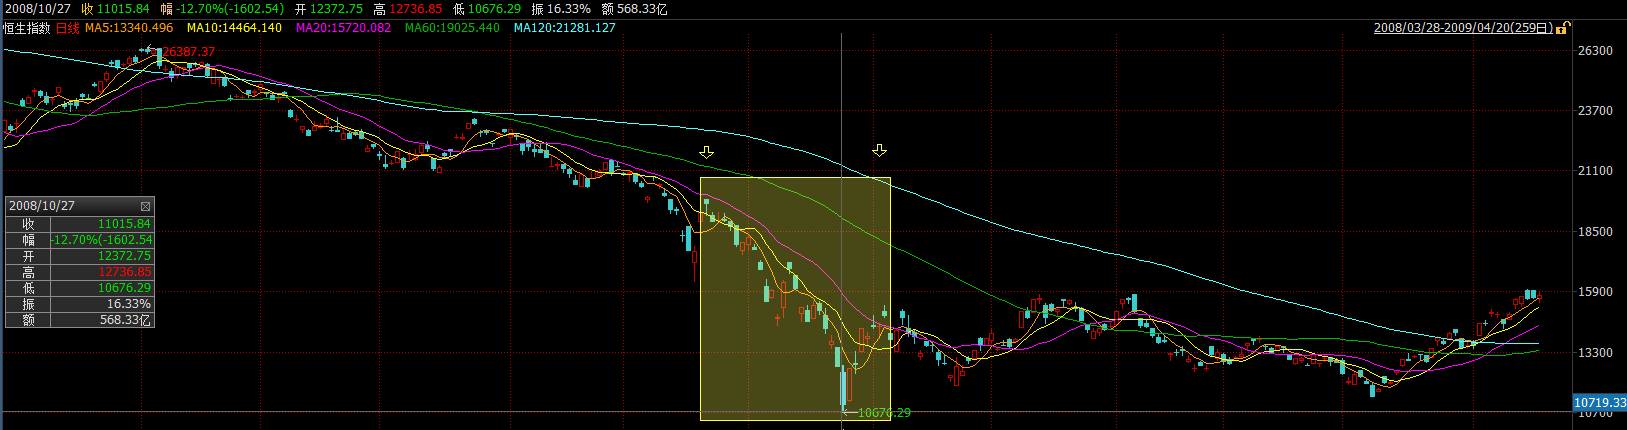
\includegraphics[width=0.9\textwidth]{img/44.png}%插入图片,按图片原尺寸插入
		\caption{恒生指数K线图14}
	\end{figure}
	
	\item 2008-11-05 $\sim$ 2008-12-11
	
	反弹后继续下跌,基本跌到底部,之后开启09年的上涨行情。
	
	\begin{figure}[H]
		\centering
		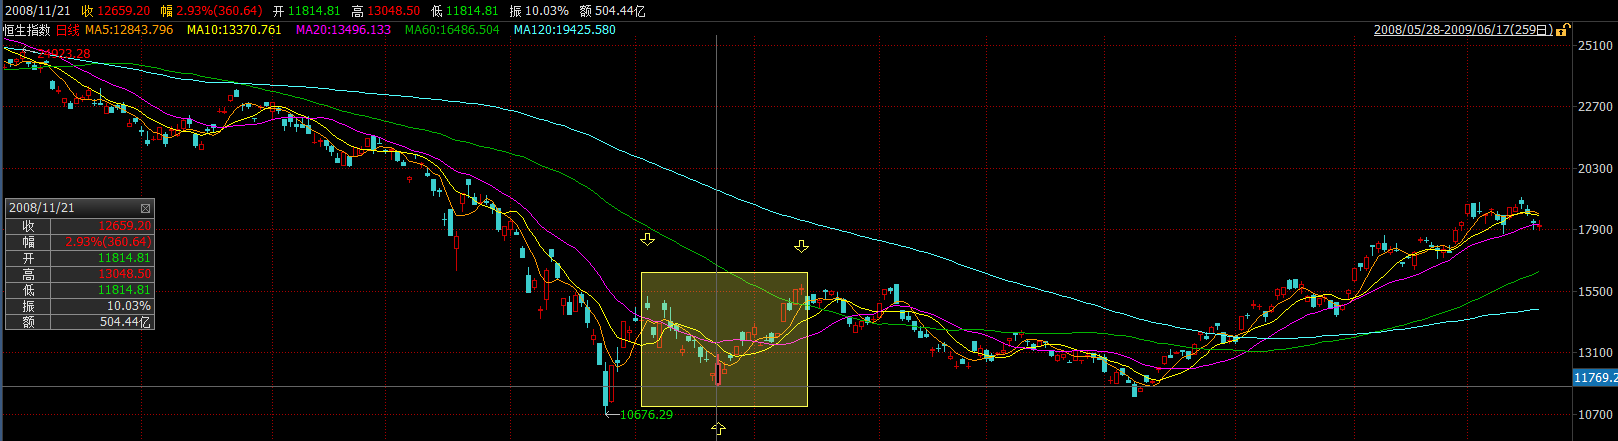
\includegraphics[width=0.9\textwidth]{img/45.png}%插入图片,按图片原尺寸插入
		\caption{恒生指数K线图15}
	\end{figure}
	
	\item 2009-01-07 $\sim$ 2009-02-10
	
	继续下跌,开始筑底,最低点比先前的最低点要高。
	
	\begin{figure}[H]
		\centering
		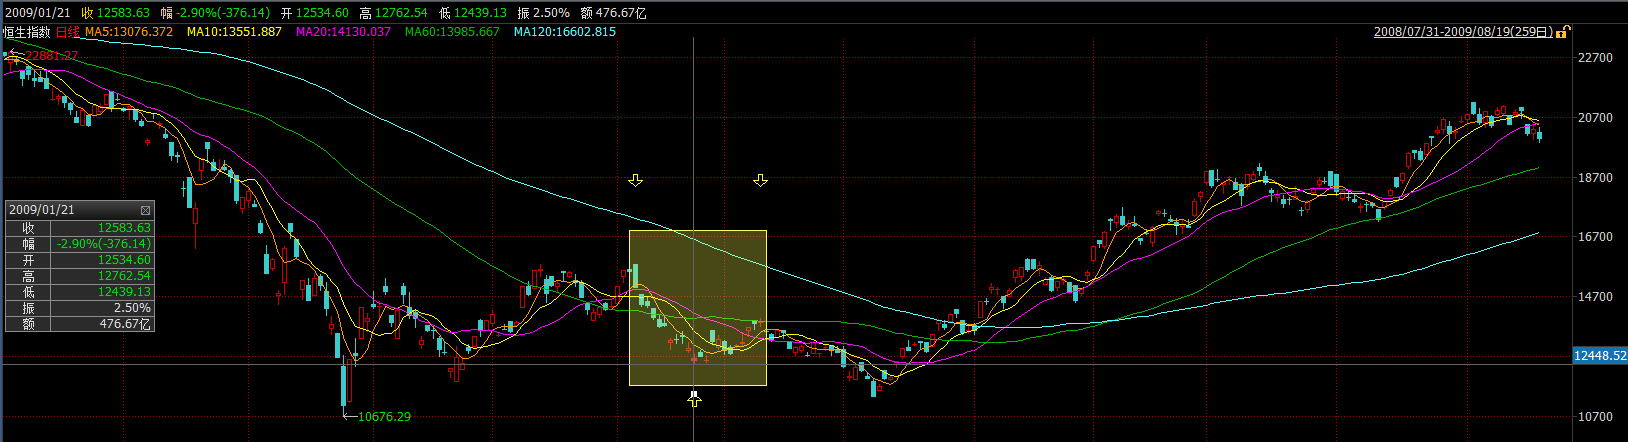
\includegraphics[width=0.9\textwidth]{img/46.png}%插入图片,按图片原尺寸插入
		\caption{恒生指数K线图16}
	\end{figure}
	
	
\end{enumerate}


\subsubsection{标普500}

	\begin{enumerate}
		\item 2001-02-06 $\sim$ 2001-03-27 
			\begin{itemize}
				\item  互联网泡沫开始破灭,处于下跌趋势中。
				\item  加息政策
			\end{itemize}
		
		\begin{figure}[H]
			\centering
			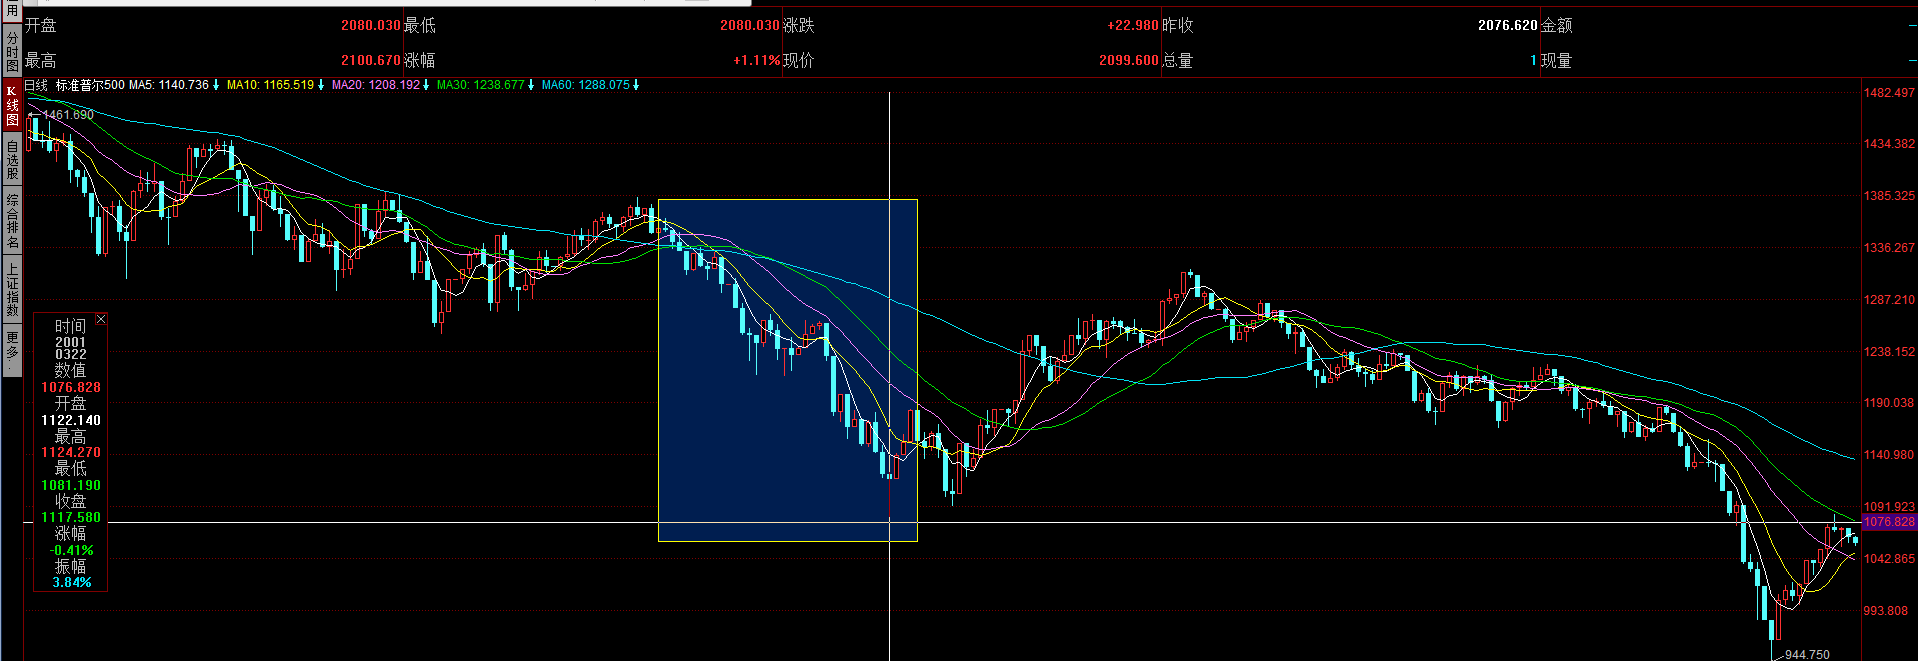
\includegraphics[width=0.9\textwidth]{img/51.png}%插入图片,按图片原尺寸插入
			\caption{K线图1}
		\end{figure}
		
		\item 2001-08-27 $\sim$ 2001-10-17
		
		“911”事件引起快速暴跌。
		
		\begin{figure}[H]
			\centering
			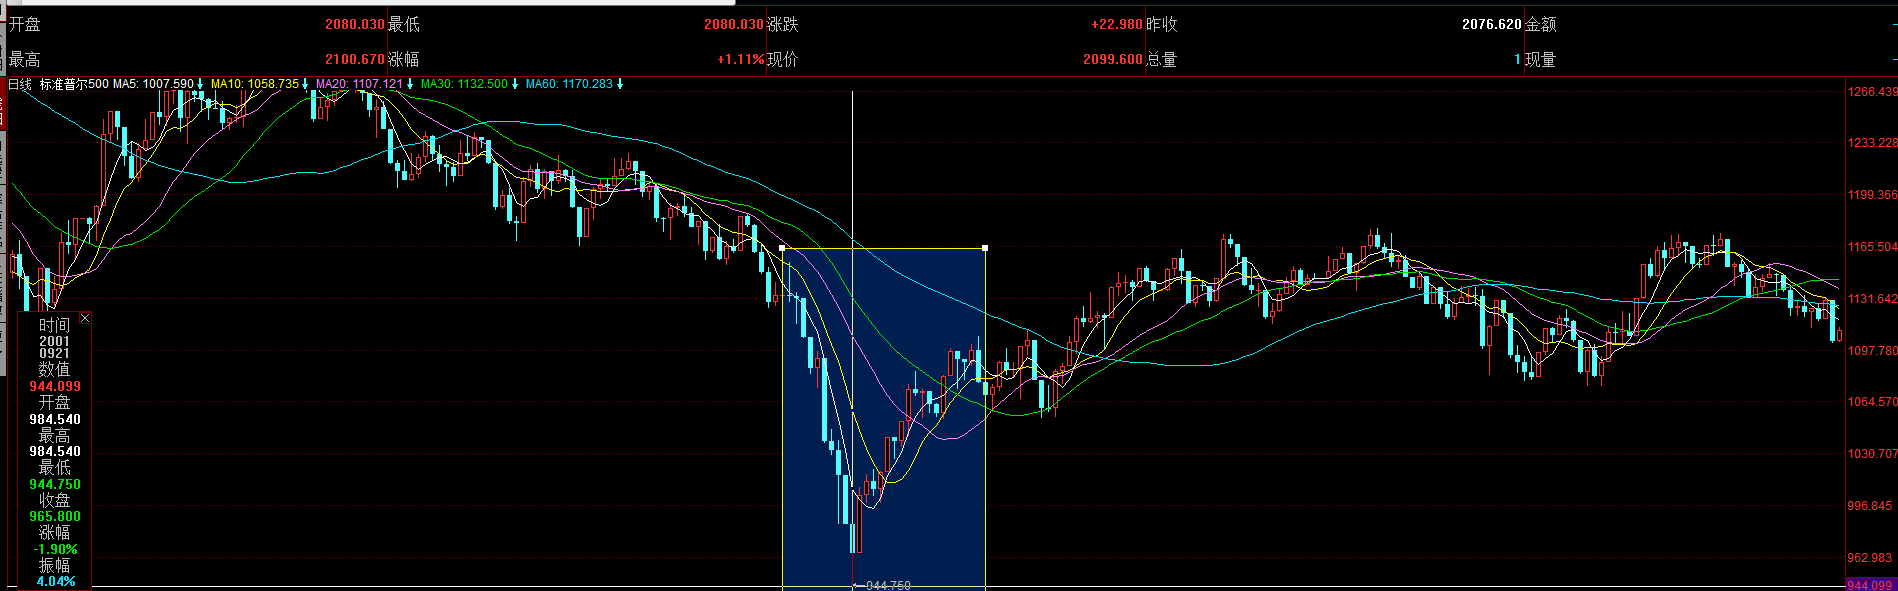
\includegraphics[width=0.9\textwidth]{img/52.png}%插入图片,按图片原尺寸插入
			\caption{K线图2}
		\end{figure}		
		
		\item 2002-06-18 $\sim$ 2002-07-31
		
		安然公司和世界通讯公司财务丑闻和信任危机。
		
		\begin{figure}[H]
			\centering
			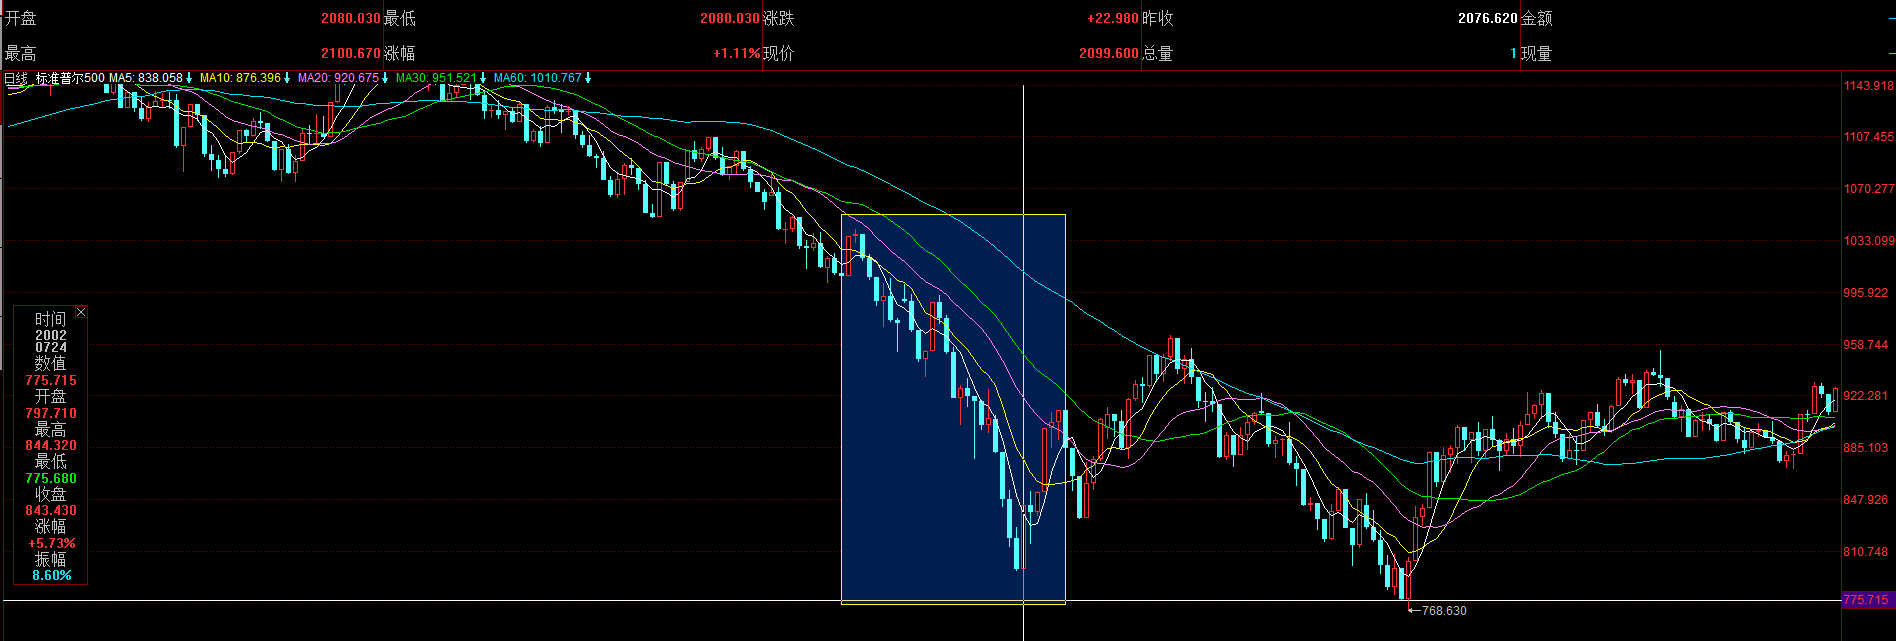
\includegraphics[width=0.9\textwidth]{img/53.png}%插入图片,按图片原尺寸插入
			\caption{K线图3}
		\end{figure}
		
		\item 2008-09-19 $\sim$ 2008-11-04
		
		全球金融危机
		
		\begin{figure}[H]
			\centering
			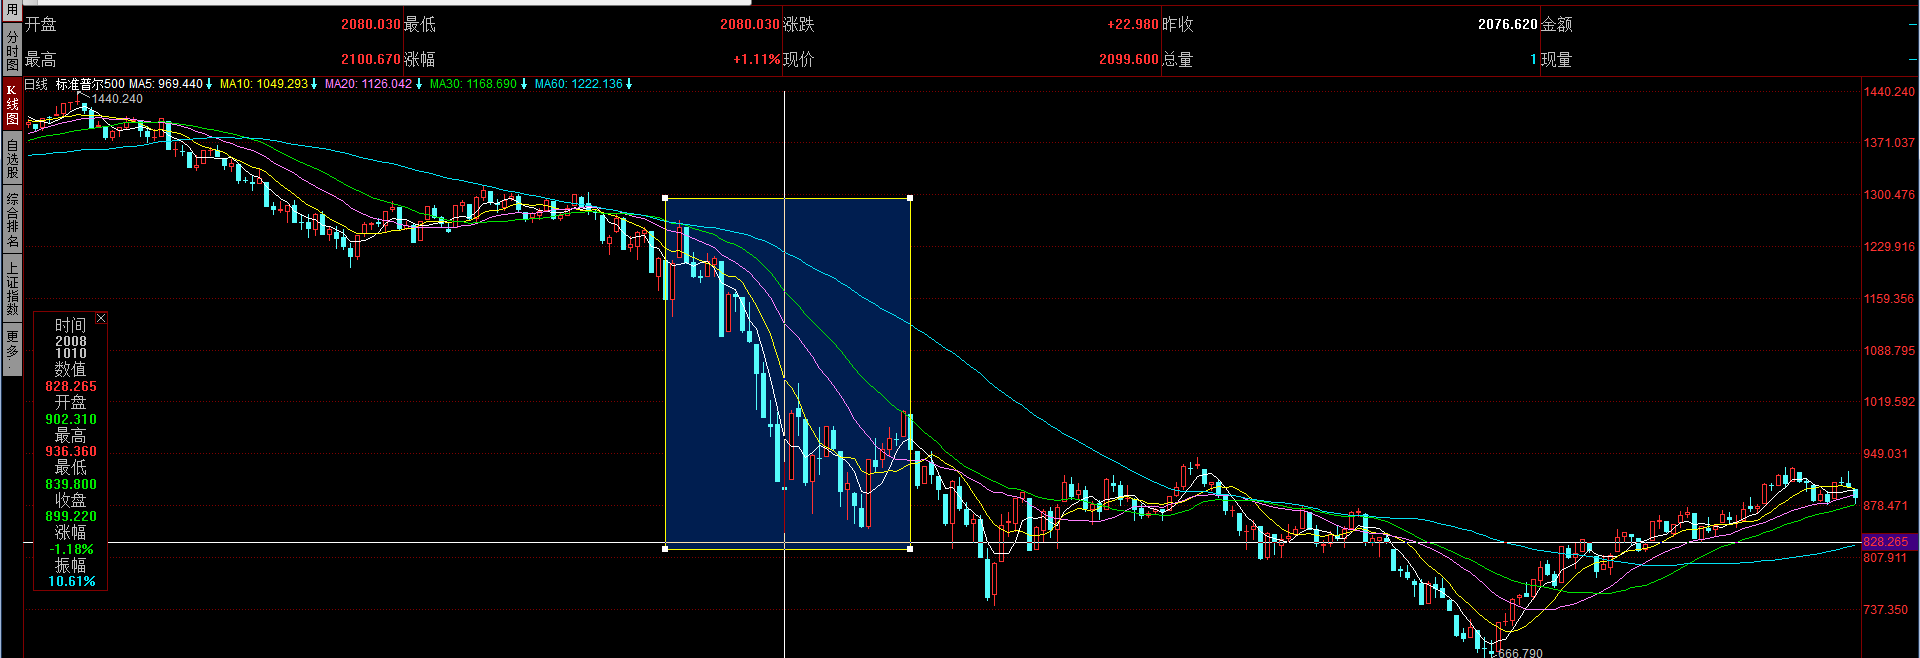
\includegraphics[width=0.9\textwidth]{img/54.png}%插入图片,按图片原尺寸插入
			\caption{K线图4}
		\end{figure}
		
		
		\item 2008-11-04 $\sim$ 2008-11-28

		全球金融危机
		
		\begin{figure}[H]
			\centering
			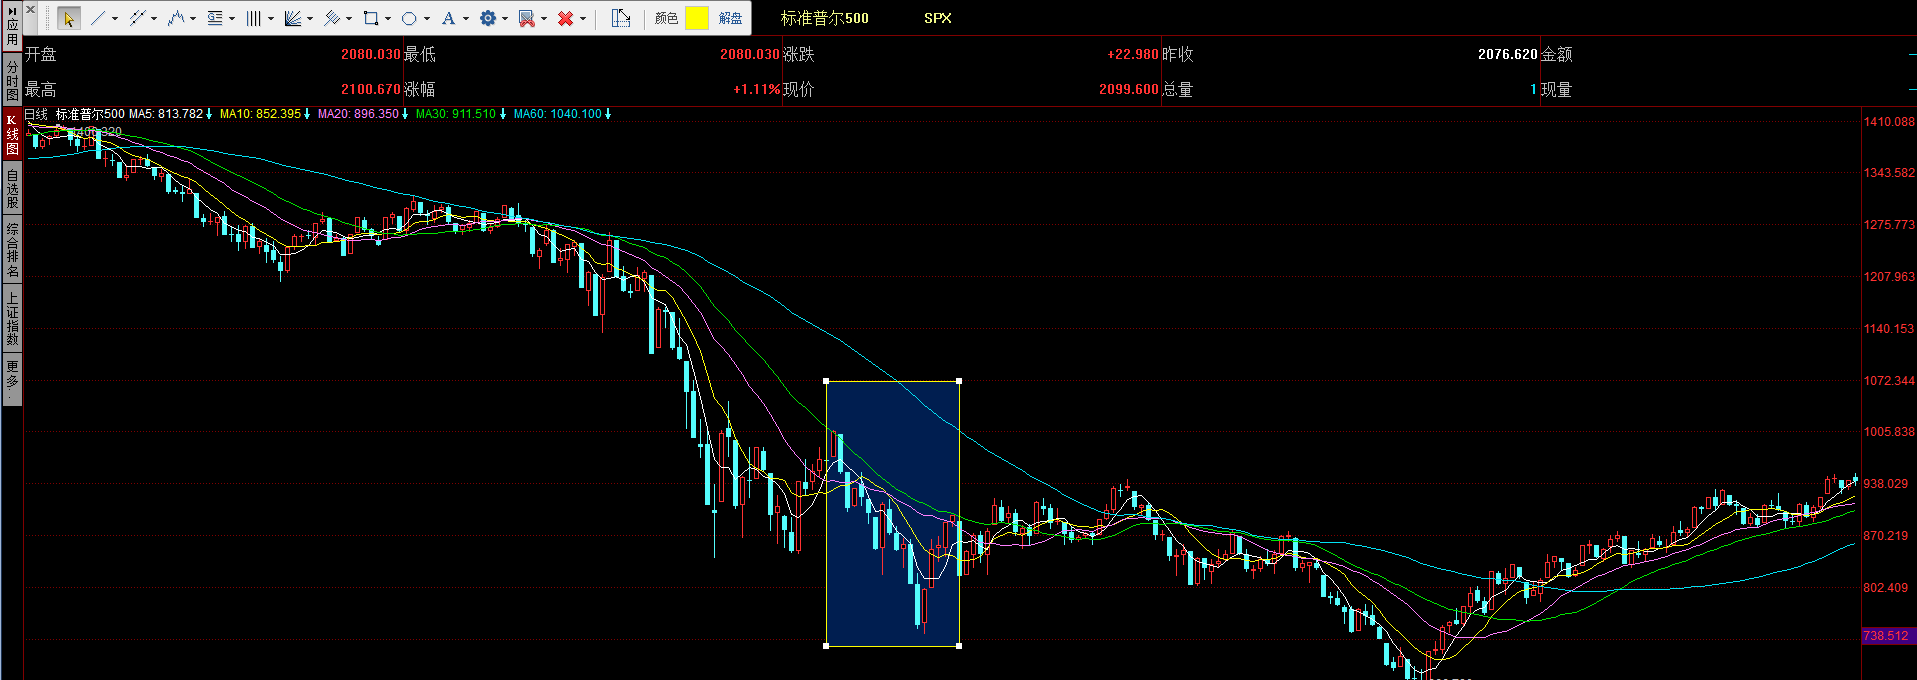
\includegraphics[width=0.9\textwidth]{img/55.png}%插入图片,按图片原尺寸插入
			\caption{K线图5}
		\end{figure}
		
		
		\item 2009-02-09 $\sim$ 2009-04-17
		
		下跌通道,基本跌到底部。之后开启09年的反弹行情。
		
		\begin{figure}[H]
			\centering
			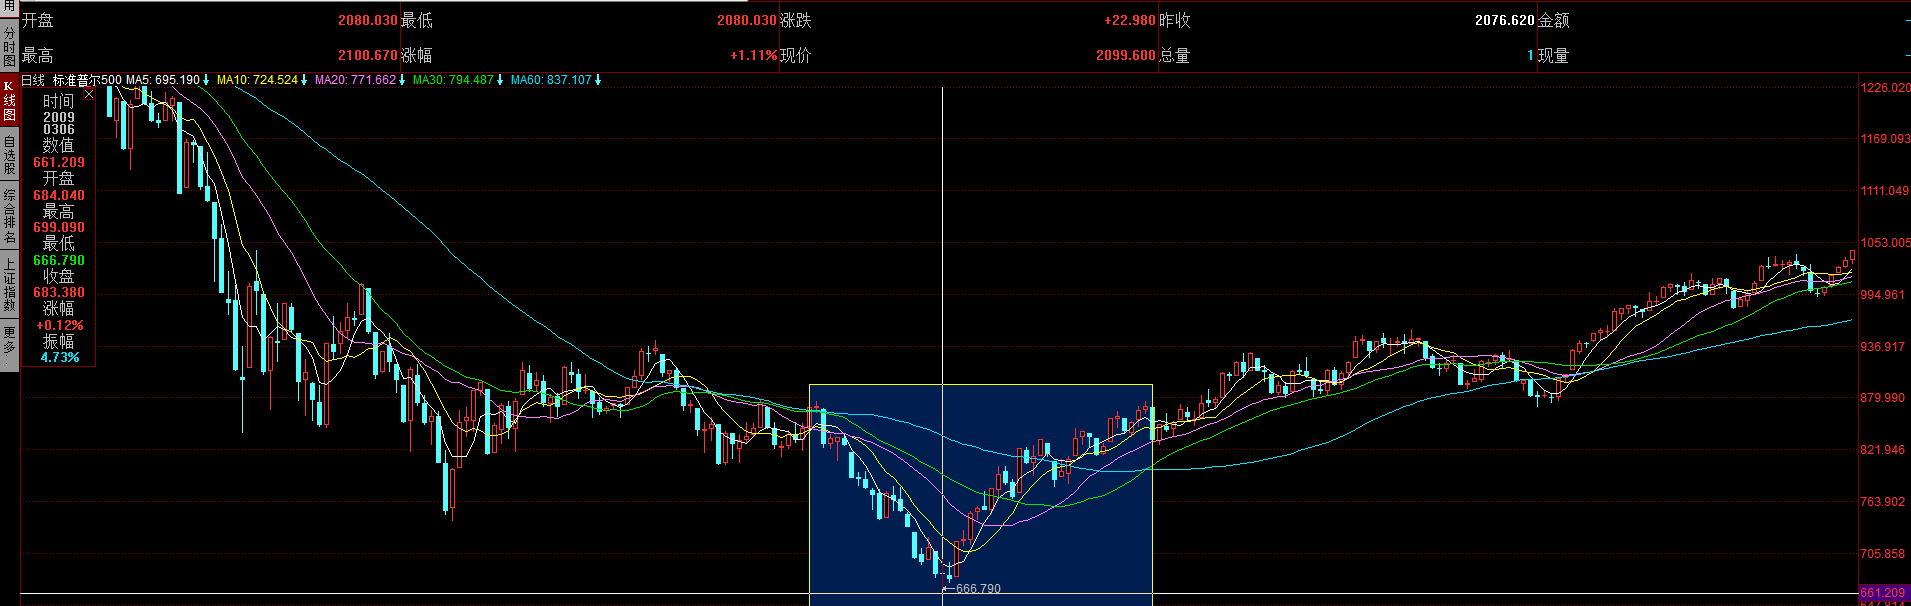
\includegraphics[width=0.9\textwidth]{img/56.png}%插入图片,按图片原尺寸插入
			\caption{K线图6}
		\end{figure}
	
	\end{enumerate}

\subsection{小结}

	\begin{itemize}
		\item 根据回测结果,满足我们定义的下跌和反弹不多,历史上还有不少快速下跌没能找到,但是我们所找到的绝大多数都是快速下跌(97年、07年都找到了多个“下跌”),个别是缓慢下跌。
		\item 符合我们的定义的下跌,大都出现在下跌趋势中,“股灾”是尤为明显。从结果中可以看出,97年的恒生指数、07$\sim$ 08年的三大指数均多次出现我们定义的“下跌”;有几例是出现在筑底反弹时;基本没有处于上涨趋势中的。那么有理由可以这样假设:如果在一段较长的时间内,多次出现我们定义的“下跌”,那么可以认为指数处于一个较长、较大的下跌通道中。
		\item 三大指数出现“下跌”的次数差距较大。如果只考虑2000年之后,那么上证指数中出现的最多,有12次,恒生指数出现8次,标普500出现6次。我暂时还想不出可能能够解释该现象的原因。
	\end{itemize}



\end{document}